\documentclass{cernrep}
\usepackage{hyperref}
\hypersetup{colorlinks,urlcolor=blue}

\begin{document}
%editors: J. Bendavid & L. Gray & P. Meridiani
\title{CMS MIP Timing Detector Simulation and Reconstruction}
\author{A. Benaglia, J. Bendavid, M. Casarsa, F. Cossutti, L. Gray, A. Li, B. Marsh, C. Neu, F. Monti, P. Meridiani, S. Pigazzini, B. Tannenwald}
\begin{abstract}
This note describes the first implementation of the CMS MIP timing detector (MTD) full simulation and reconstruction as implemented for the Technical Design Report TDR-19-001.
\end{abstract}

\maketitle
\tableofcontents
\section{Introduction}
This analysis note describe the first implementation in full simulation of the MIP Timing detector (MTD) simulation and reconstruction.

The note starts describing the simulation geometry in~\ref{sec:sim} as implemented for the MTD Technical Design Report. The simulation of the readout electronics, based on design available during the TDR, is described in section~\ref{sec:digi}.

Few key performance aspects are then described in~\ref{sec:acceptance}. Energy deposition, efficiency and occupancy for the 2 compartments of the detector, the Barrel Timing Layer (BTL) and the Endcap Timing Layer (ETL) are discussed in detail for single gun events and minimum bias events.

\section{Simulation and Digitisation}
\section{Reconstruction of deposited energy and time in the MTD}
%editors: P. Meridiani & A. Benaglia
\label{C5Sec:mtdreco}
%\subsubsection{Energy and time reconstruction}
The energy deposited by a particle is reconstructed by clustering the energy deposits in adjacent cells matched to a track.  
A basic algorithm consists in summing the energy deposits -- above the readout threshold -- that lie within a cone of $\Delta R = 0.05$ around the extrapolation of track to the MTD surface. 
%[Note: this description is valid for the current plots. Text and the plots need to be updated to reflect the usage of clusters]. 
The distributions of the total energy deposit predicted for single muons and pions, and for minimum bias events are shown in Fig.~\ref{fig:BTL_Edep}-left for BTL and Fig.~\ref{fig:BTL_Edep}-right for ETL. 
Muons behave as MIP in the timing layer, and the most probable value of a Landau interpolation of the energy deposit distribution correspond to about 5~MeV in BTL and 0.15~MeV in ETL. In the case of hadrons, the distribution features a high energy tail ascribed to nuclear interactions.

\begin{figure}[hbtp]
\centering
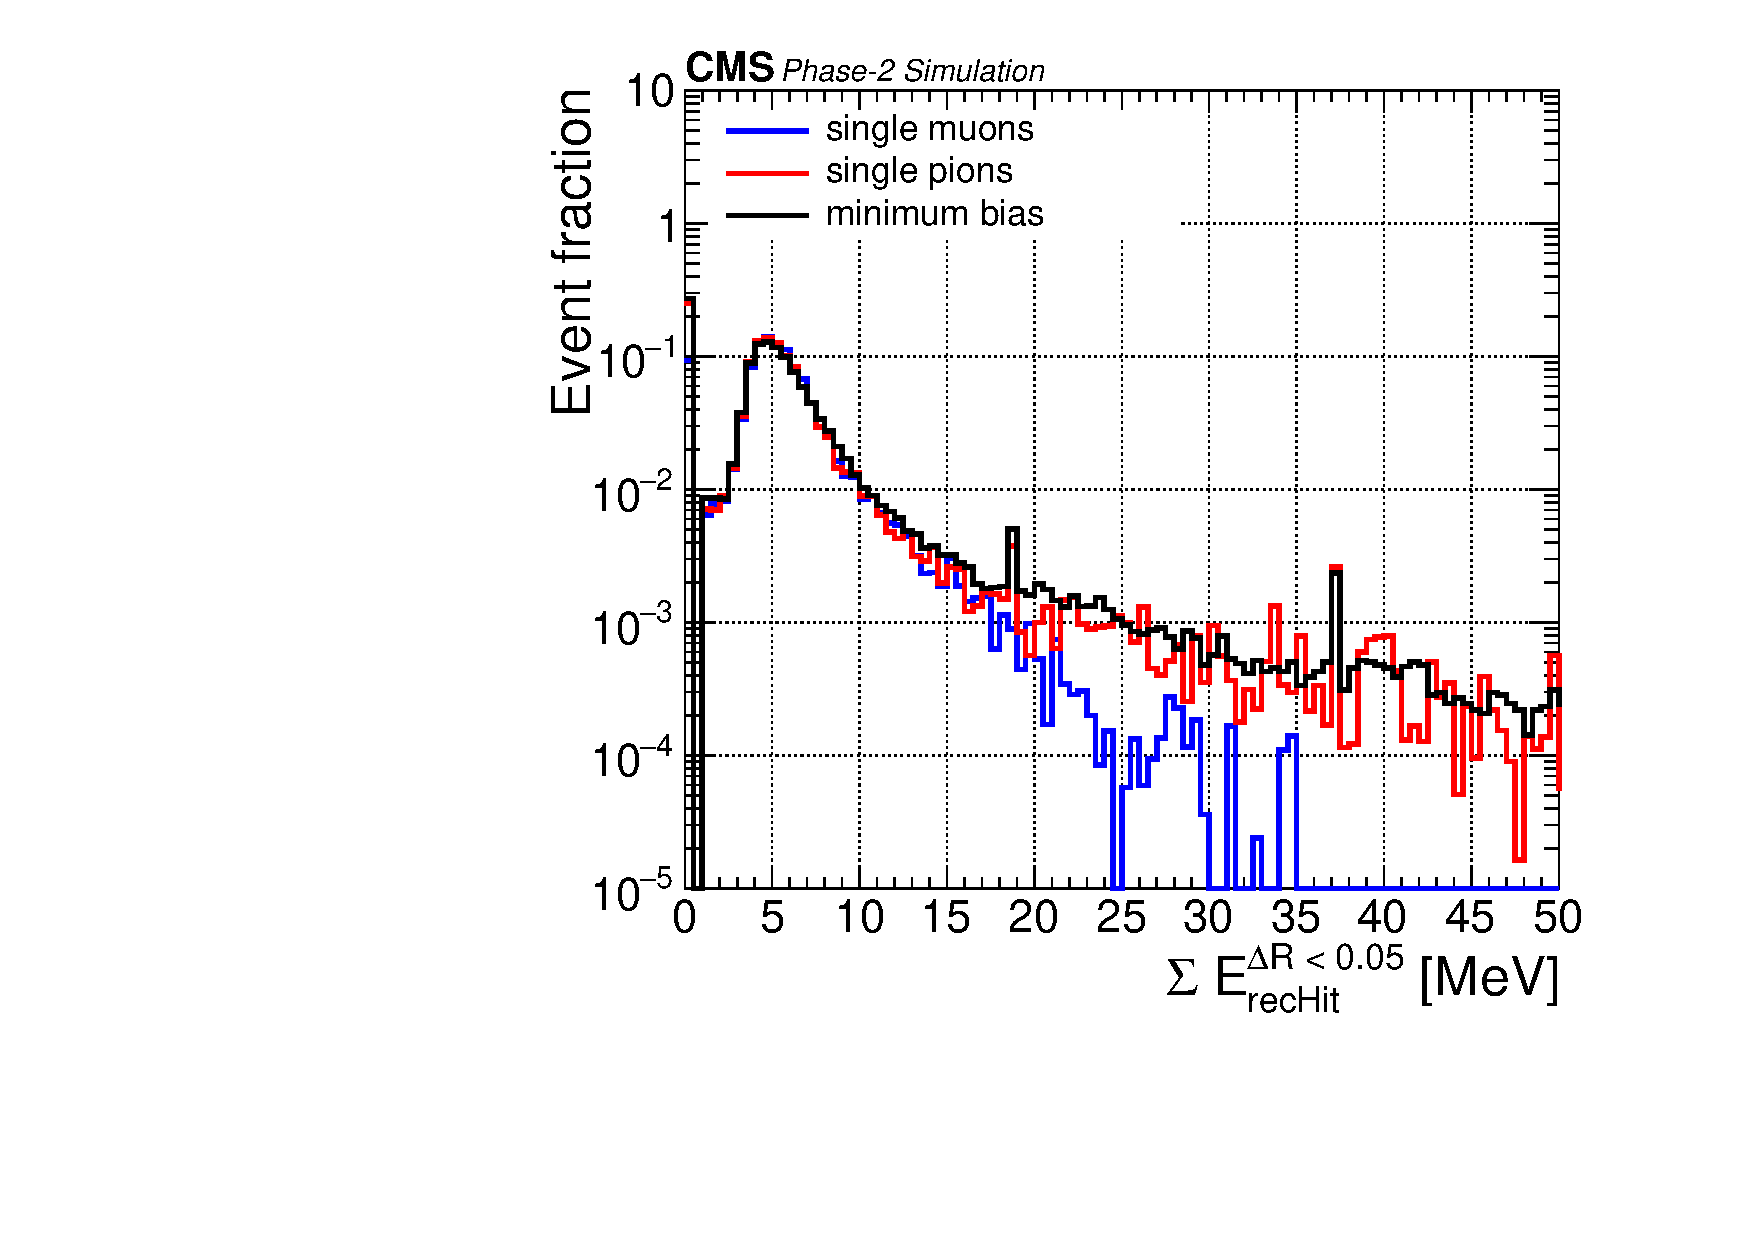
\includegraphics[width=0.49\textwidth]{fig/performance/c_all_Edep.pdf}
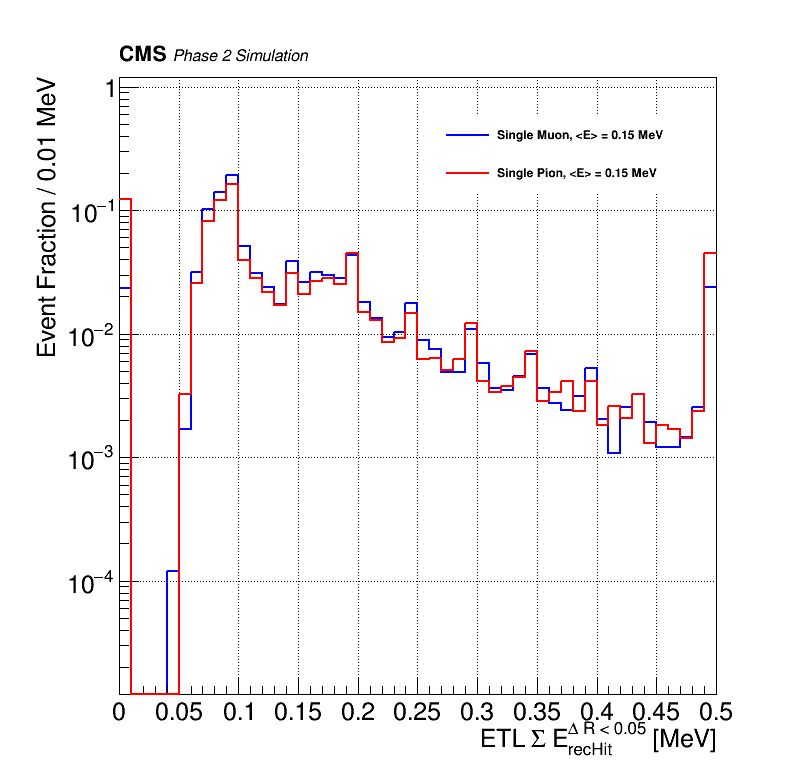
\includegraphics[width=0.45\linewidth]{fig/performance/ETL_energyDeposition.png}
%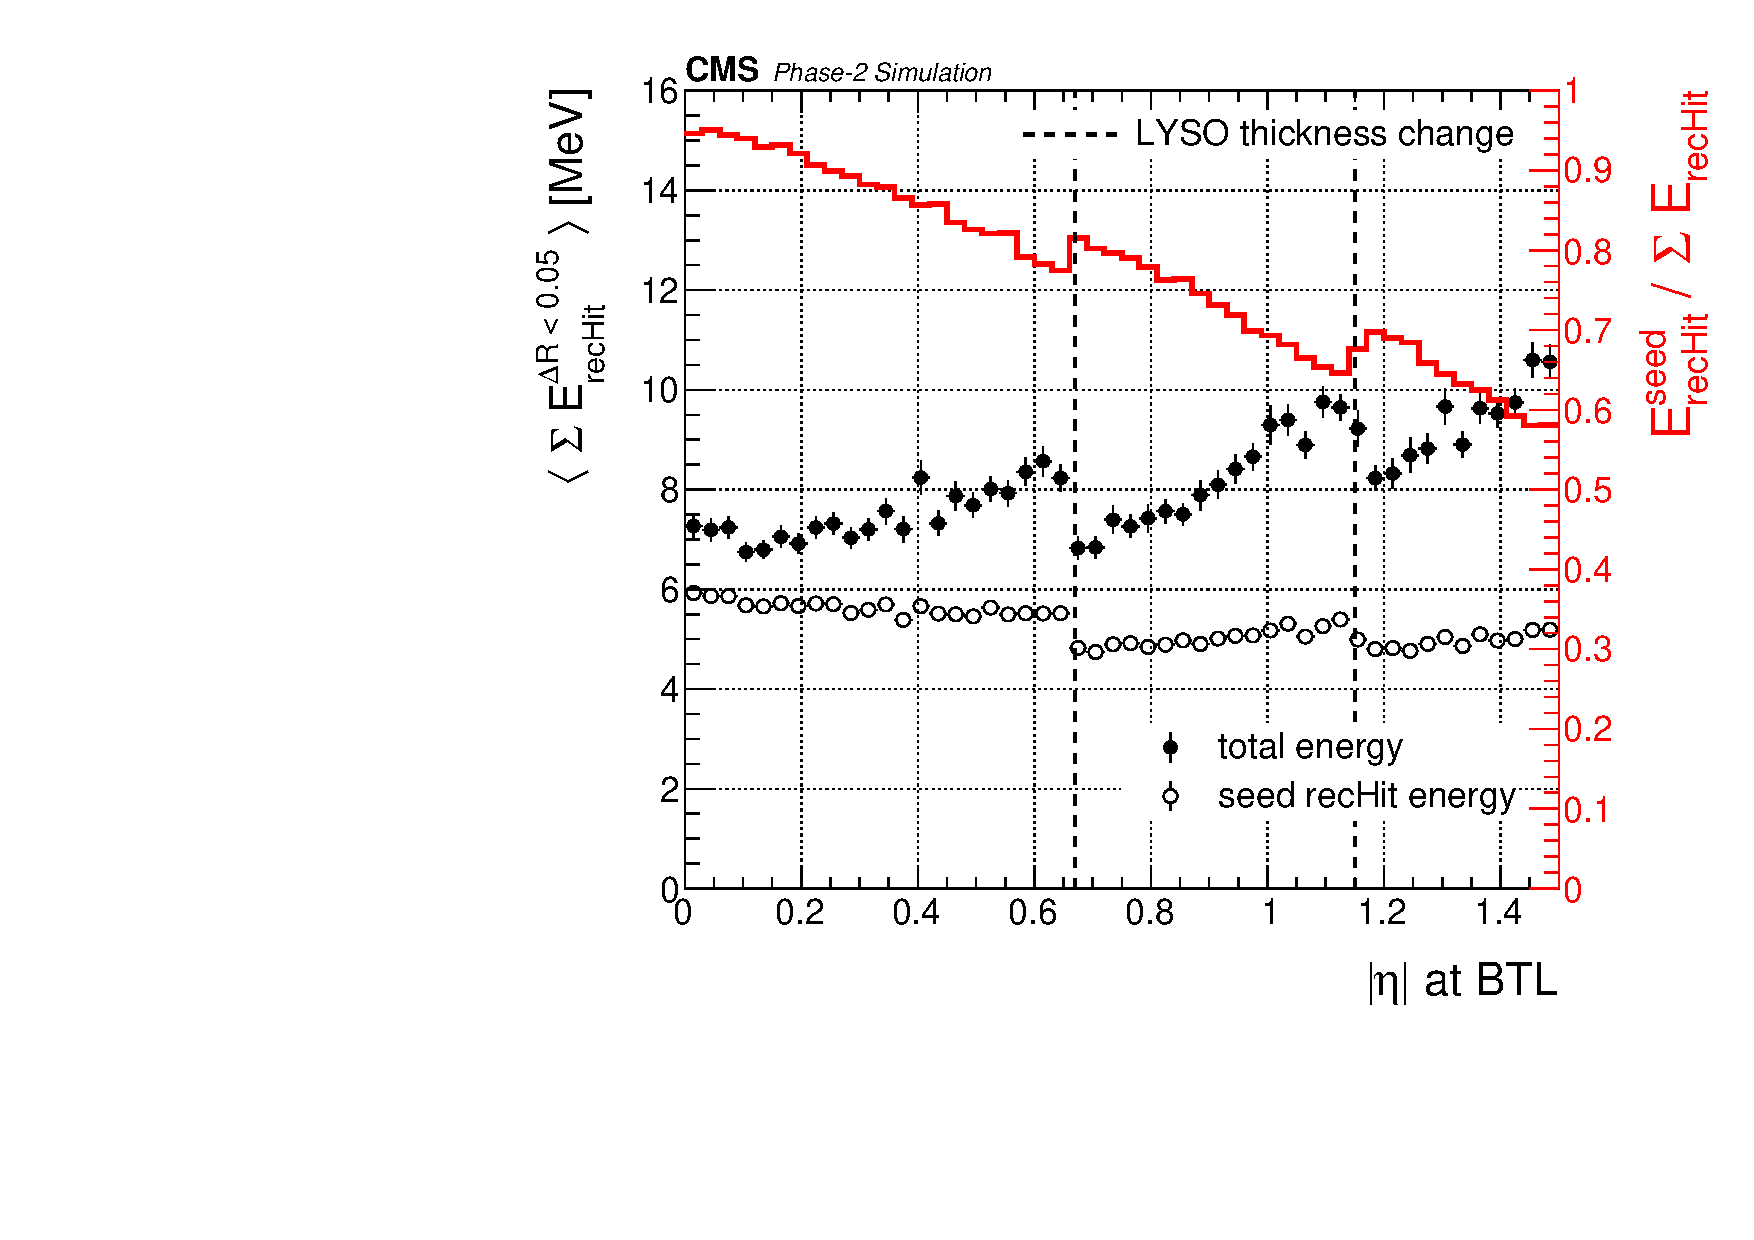
\includegraphics[width=0.48\linewidth]{fig/performance/c_minBias_maxEnergy_vs_eta.pdf}
\caption{Left: Distribution of the energy deposited in the BTL as predicted by the simulation for single muon (blue), single pion (red), and minimum bias events. 
%The energy is reconstructed as the sum of all BTL hits within a cone of $\Delta R < 0.05$ around the track propagated to the BTL front surface. 
Right: Distribution of the energy deposited in the ETL as predicted by the simulation for single muon (blue) and single pions (red). 
%The energy is reconstructed as the sum of all BTL hits within a cone of $\Delta R < 0.05$ around the track propagated to the BTL front surface. 
%on the left and minimum bias events on the right. 
In these plots, single muon and single pion events are weighted so that their $p_{T}$ and $\eta$ spectra match the ones observed for minimum bias events. 
}
%%%PM we probably need to explain the spikes which corresponds to saturation of the electronics 
\label{fig:BTL_Edep}
\end{figure}

%in the upstream material and in BTL itself [TBC]. 
The energy deposition is also shown as a function of the pseudo-rapidity for the BTL in Fig.~\ref{fig:BTL_EdepVsEta_timeRes}-left. 
This figure shows the average total energy deposited by a muon, as well as the average energy deposited in the crystal with highest energy in each cluster (``seed crystal'') and the ratio of these two quantities as a function of pseudorapidity. 
%for single muon and minimum bias events, respectively. 
The energy deposition is fairly independent as a function of $\eta$, because of the crystal slant-thickness leveling. The fraction of energy deposited in the seed crystal, shown in the same plot,  decreases as a function of $|\eta|$ to about 60\% at the end of the barrel, where tracks are more likely to cross adjacent crystals. The energy deposition is also fairly uniform in ETL, since the sensors remain the same thickness throughout the annulus covered by the detector, driven by the need to keep the
depleted region of the silicon sensors thin to reduce the impact of
Landau fluctuations on the sensor's timing resolution.
%The effect of crystal thickness leveling in three pseudorapidity regions reflects in the equalization of the average total energy deposit along $\eta$. 
%Because of the crystal arrangement, inclined tracks at high $\eta$ are likely to cross multiple adjacent crystals, so that the fraction of energy deposited in the most energetic of them decreases, on average, to about 60\% at the end of the barrel.

\begin{figure}[hbtp]
\centering
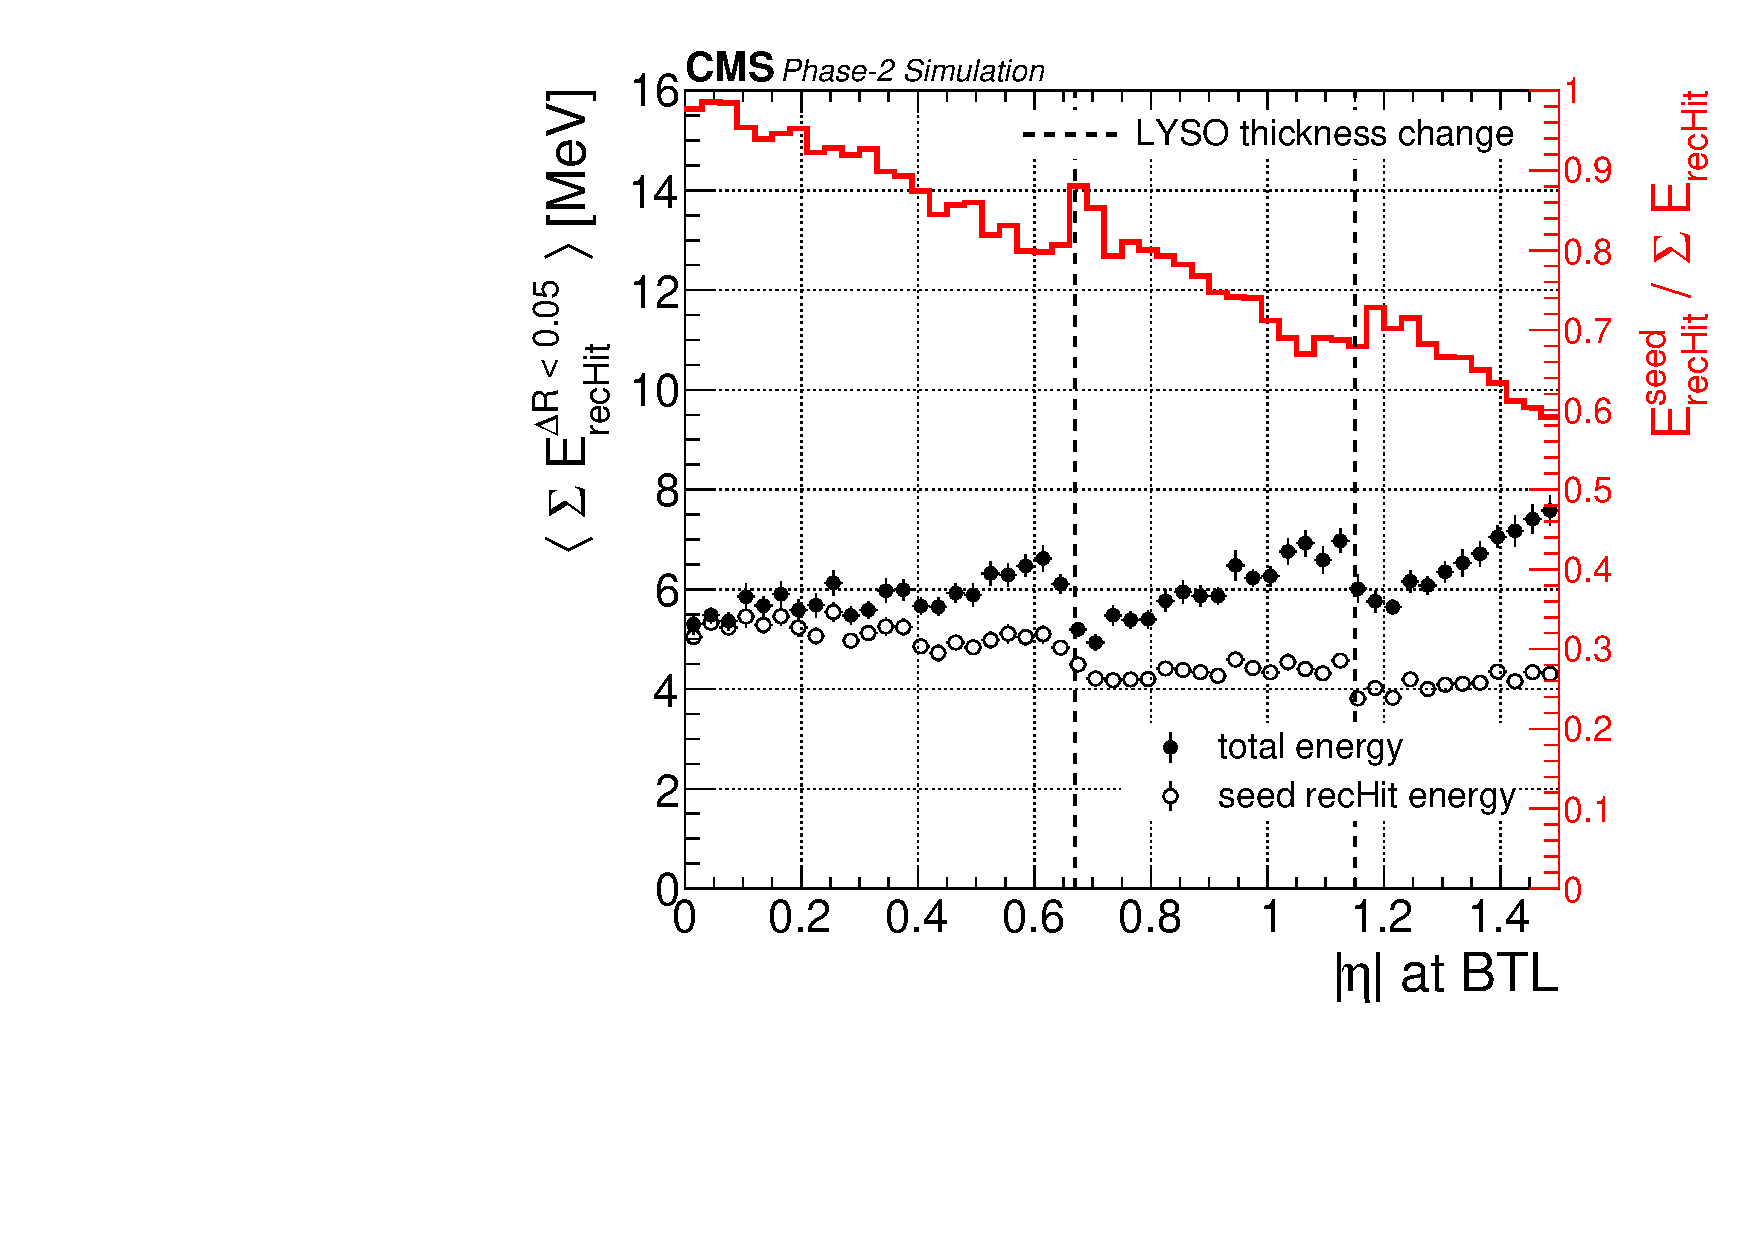
\includegraphics[width=0.49\linewidth]{fig/performance/c_singleMuPtFlat_maxEnergy_vs_eta.pdf}
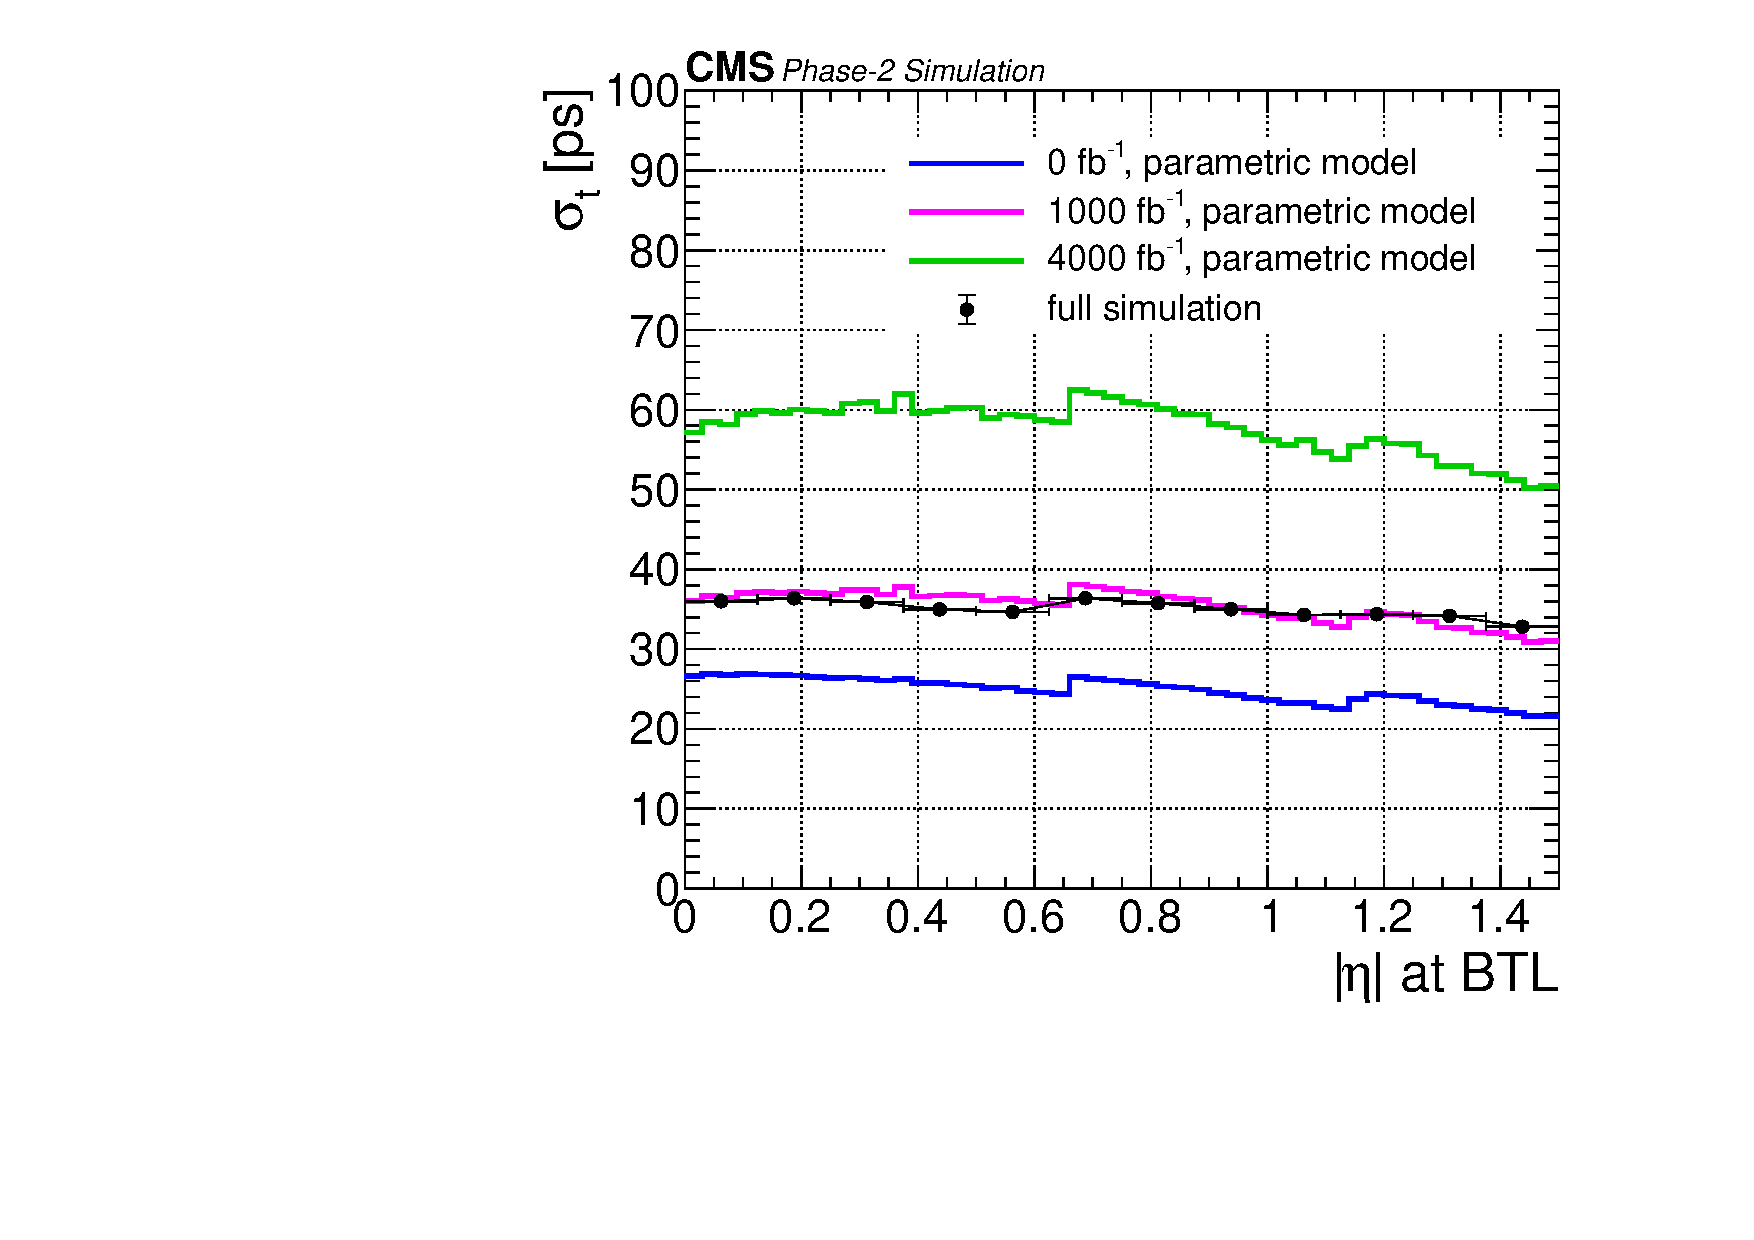
\includegraphics[width=0.49\textwidth]{fig/performance/c_MinBias_timeRes_vs_eta.pdf}
\caption{Left: Average total energy deposit (black solid dots), energy of the seed crystal (empty dots) and ratio of the two above quantities (red line, right axis) as a function of pseudorapidity, for single muon events. Right: Average time resolution for clusters associated to tracks in minimum bias events for three ageing scenarios corresponding to 0 (blue), 1000 (purple), and 4000~fb$^{-1}$ (green). The prediction of the parametric model compared to the full simulation for 1000 fb$^-1$.
}
%%%PM we probably need to explain the spikes which corresponds to saturation of the electronics 
\label{fig:BTL_EdepVsEta_timeRes}
\end{figure}

%[Discuss amplitude walk correction here?]

%[Text taken from 2.1.1.1]

The time measurement associated to a cluster is obtained
from the average of single-hits time measurements, weighted on the
respective resolutions.  In BTL the time measurement for a single crystal is
obtained from a linear combination of the left and the right SiPMs
measurements, $t_{\text{ave}} = C_{L} \cdot t_{L} + C_{R} \cdot t_{R }$; where $C_{L}$
and $C_{R}$ are two calibration coefficients that can be  
derived in situ. According to test beam results for particles at
normal incidence (Section~2.1.1), the time measurement is independent
of the track impact point along the crystal for $C_{L} = C_{R} = 0.5$.  
These values are adopted in the current simulation and in the studies
reported in this TDR.  

The expected average time resolution for clusters associated to
tracks in minimum bias events is shown for BTL Fig.~\ref{fig:BTL_EdepVsEta_timeRes}-right 
for three ageing scenarios corresponding to 0, 1000, and
4000~fb$^{-1}$. The response evolution is parameterized according
to the model described in Section~2.1, normalized to test beam 
results by means of a \GEANT simulation of the test beam setup. 

%
%The energy distribution profiles of Fig.~\ref{fig:BTL_Edep} allow the performance of the BTL in time reconstruction to be predicted as a function of the pseudorapidity, as shown in Fig.~\ref{fig:BTL_timeRes} for three different aging scenarios corresponding to 0, 1000, and 4000~fb$^{-1}$. The single sensor timing resolution for the unaged detector and a 2.6 MeV most probable energy deposit in one crystal is assumed to be 43 ps, as measured in beam tests. This number is then scaled by the actual energy deposit predicted by the simulation, and other contributions to the timing resolution -- the DCR term being the dominant one -- are added in quadrature, according to the parametric model described in Sec.~2.1. The timing resolution as predicted by the full simulation is also superimposed. In the plots, the timing resolution is shown after combining the individual resolutions expected in each crystal of the cluster.   
%
The average per-track resolution for tracks with the \pt spectrum of 
minimum bias events is \tres or better across the full BTL acceptance up to 
1000~fb$^{-1}$, while it drifts to \trend at the end of  operations.  
The average resolution during the HL-LHC operation (2000 fb$^{-1}$) is 
about 40~ps. The results from the full simulation corresponding to
1000~fb$^{-1}$ are used as a reference for physics studies. 


%\subsubsection{ETL}

%The energy deposited by a particle in the ETL is reconstructed adding
%all the information of all cells above the readout threshold that lie
%within a cone of $\Delta R = 0.03$ around the extrapolation of track
%to the ETL surface. 
%[NB: As with BTL, this description is valid for the current plots. Text and the plots need to be updated to reflect
%the usage of clusters].  
%The distribution of the total energy deposit
%predicted by the full simulation of single muon, single pion and
%minimum bias events is reported in the top panel of
%Fig.~\ref{fig:ETL_Edep}. Muons behave as MIP in the timing layer, and
%their most  probable and average energy deposit correspond to about X
%and Y.Y MeV, respectively. Hadrons, instead, show a larger total
%energy deposit of about Z MeV due to high energy tails from
%interactions  in the tracker. The average total energy deposit in ETL,
%as well as the average energy deposited in the seed pad of each ETL
%cluster and the ratio of these two quantities, are reported in the
%central and bottom panels of Fig.~\ref{fig:ETL_Edep} as a function of
%pseudorapidity, for single muon and minimum bias events,
%respectively..

%\begin{figure}[hbtp]
%\centering
%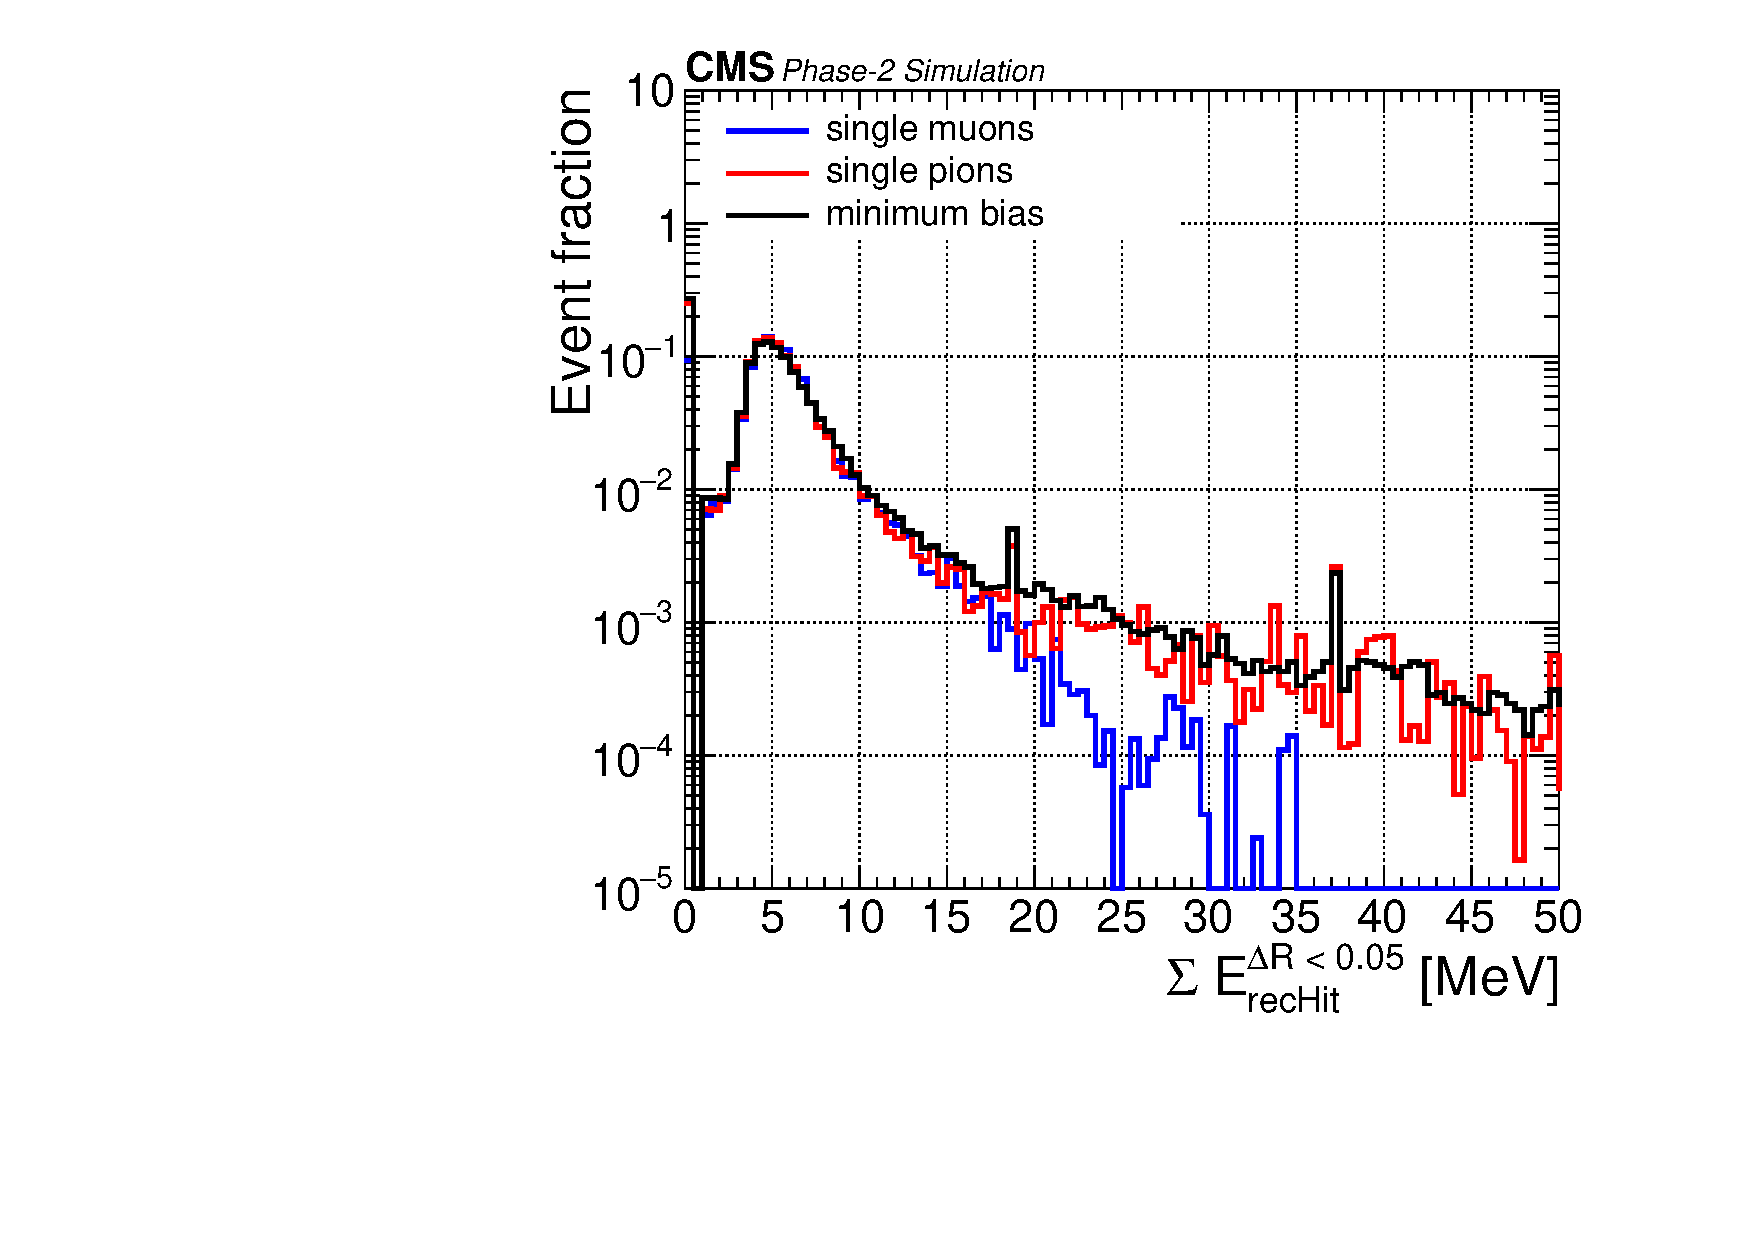
\includegraphics[width=0.48\textwidth]{fig/performance/c_all_Edep.pdf}
%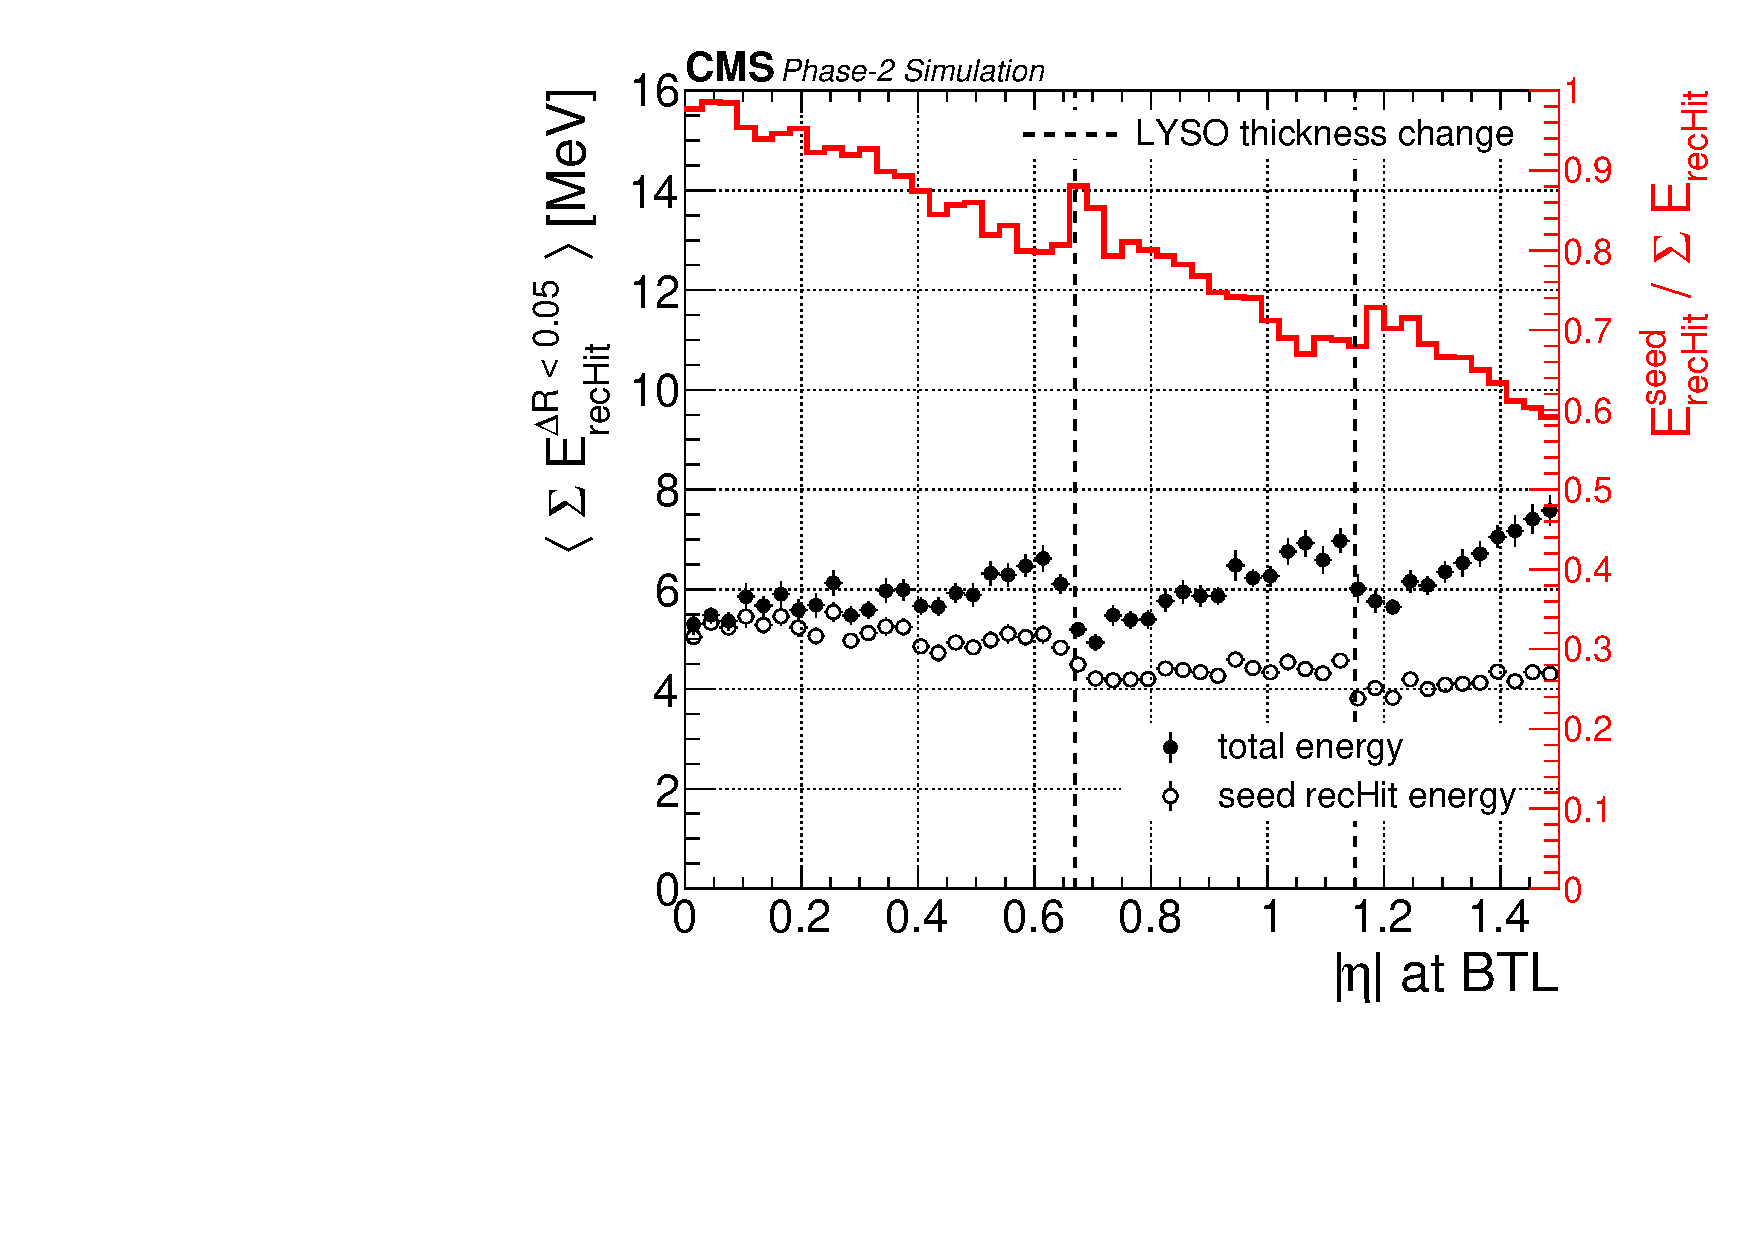
\includegraphics[width=0.48\linewidth]{fig/performance/c_singleMuPtFlat_maxEnergy_vs_eta.pdf}
%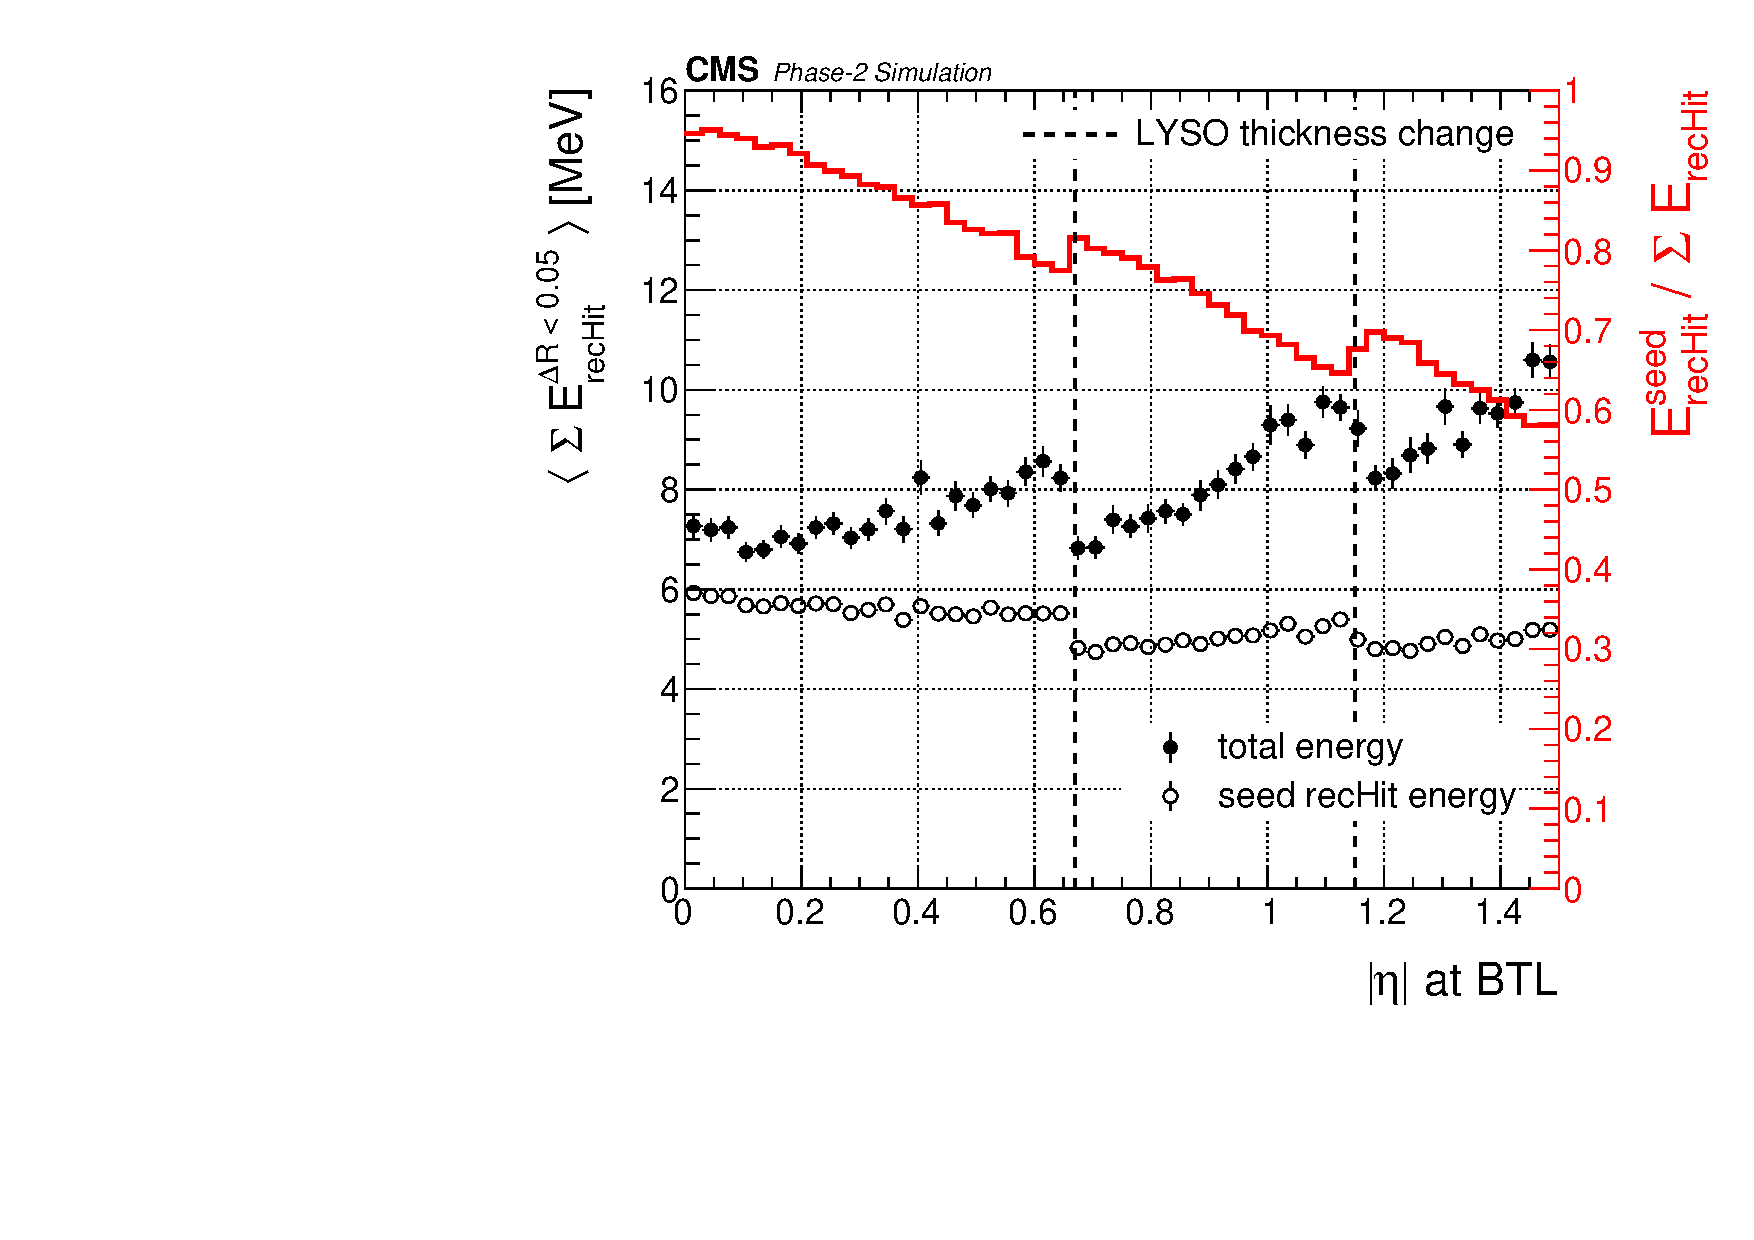
\includegraphics[width=0.55\linewidth]{fig/performance/c_minBias_maxEnergy_vs_eta.pdf}
%\caption{FIXME - ETL PLOTS Left: distribution of the energy deposited in the ETL as predicted by the simulation for single muon (blue), single pion (red), and minimum bias events. The energy is reconstructed as the sum of all ETL hits within a cone of $\Delta R < 0.02$ around the track propagated to the ETL front surface. Right: average total energy deposit (black solid dots), energy of the seed crystal (empty dots) and ratio of the two above quantities (red line, right axis) as a function of pseudorapidity, for single muon events.
%}
%\label{fig:ETL_Edep}
%\end{figure}

%Given the less advanced state of the electronics studies for ETL at the time of developing its simulation chain, the digitization routine for this detector is simpified to be a smearing of a threshold crossing time of simulated hits in each ETL pad with a threshold of 0.02 of the average energy deposition of a MIP in the LGAD's depleted region. The injected time resolution is 35~ps. The ETL local reconstruction accounts for the conversion of the digitizer output into hits with recorded energy and coordinate values, and prepares the hits for use in the tracking reconstruction described later in this text.

%%%PM Energy deposition for single mu, single pi and minimum bias
%%%PM Time resolution can be just a sentence given that there is just a simple smearing

\section{Clustering}

%editors: L. Gray & P. Meridiani
In the first step of the MTD track reconstruction, a simple topological clustering is performed to associate adjacent MTD hits above the readout threshold. 
%In particular, multiple hits can be associated to a single track which impacts BTL at a shallow angle, either at p$_{T}$ below 2\mathrm{GeV} or at higher pseudo-rapidity values (above $|\eta|>0.8$). 
Hits are required to be compatible in time, as this shows to mildly improve the resolution of the cluster parameters at high pile-up. The baricenter, weighted by the single hit energy, is used as an estimate of the cluster position and time. 

Comparison of the BTL cluster size and reconstructed time 
%and the cluster reconstructed position 
is shown in Figure \ref{fig:clusterMuPuComp} for single muon simulated events with an average of 200 pile-up events and without pile-up.

\begin{figure}[!h]
\centering
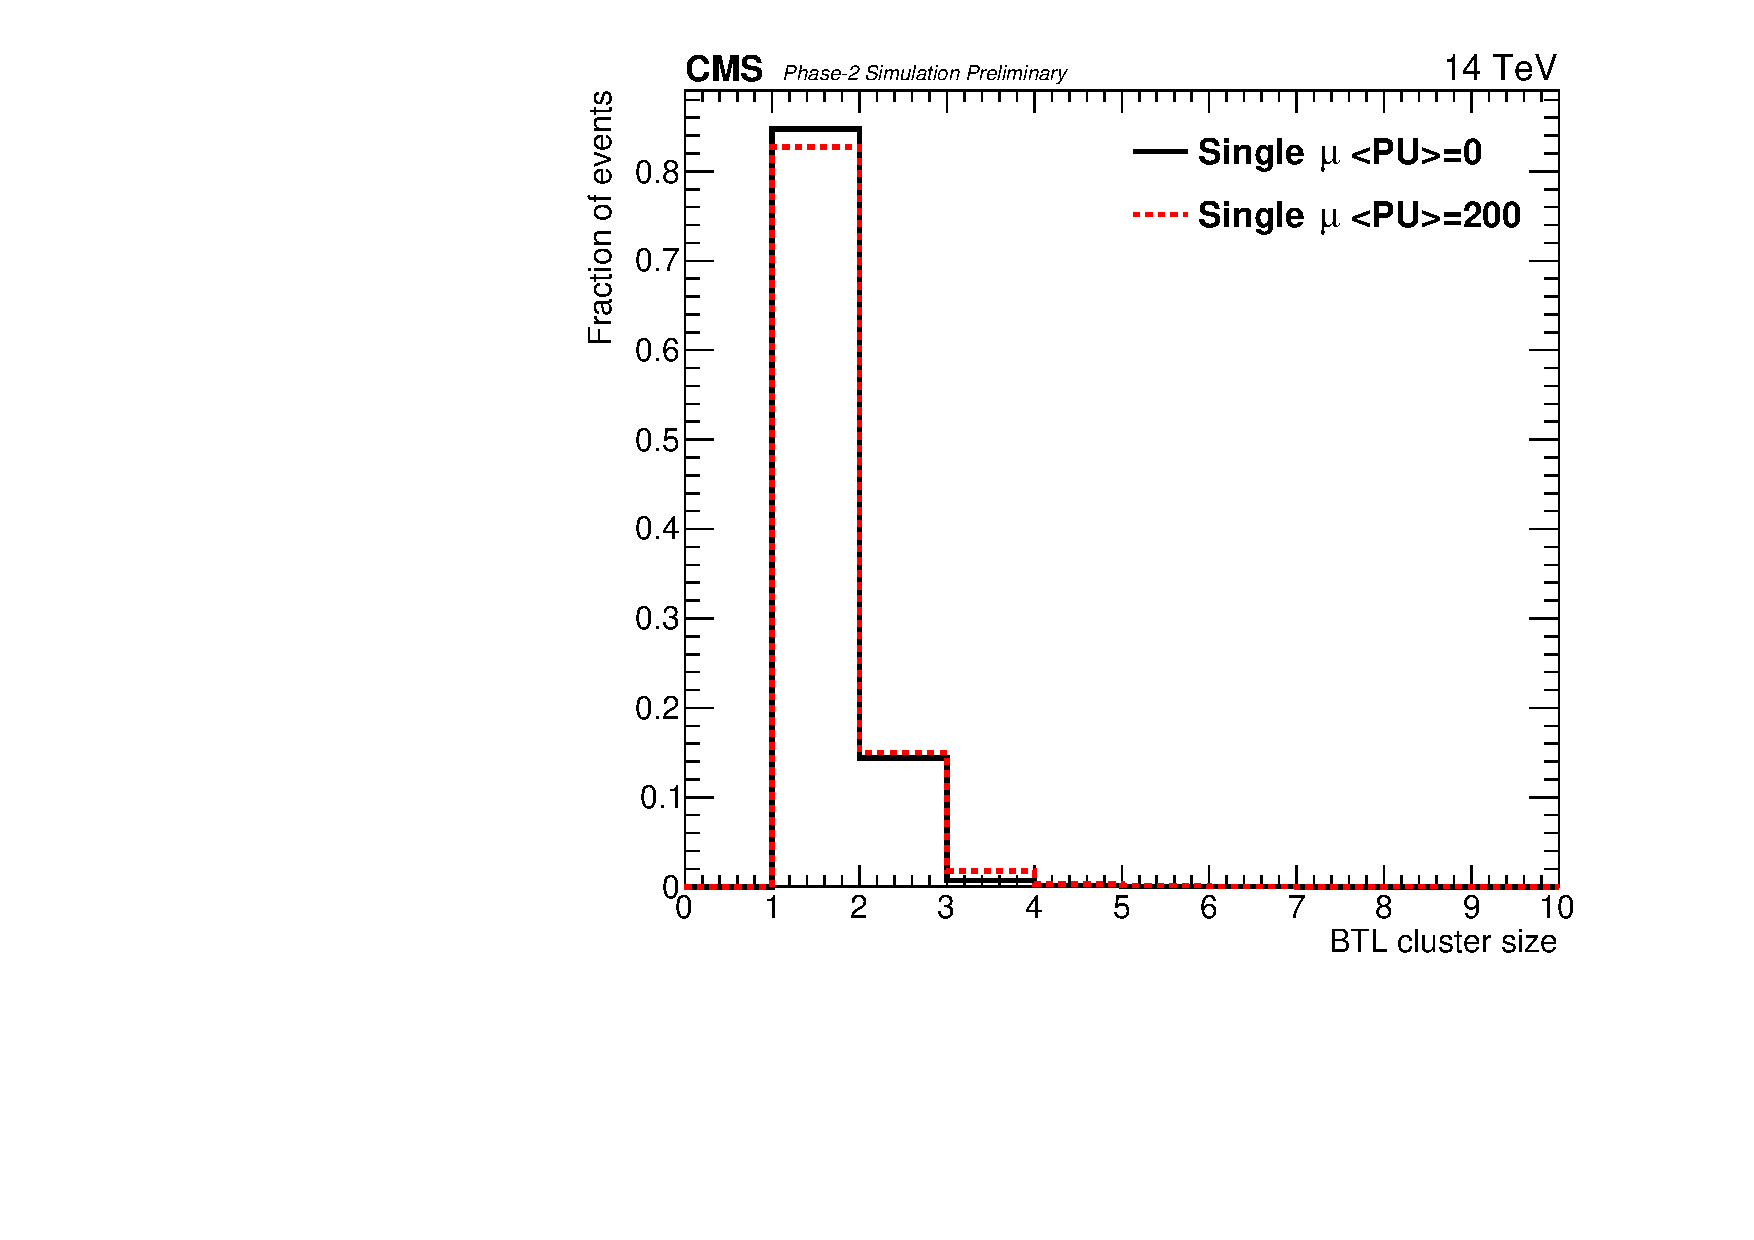
\includegraphics[width=0.48\textwidth]{fig/performance/ClusterAndTracks/BTLbestCluster_size_muPUcomp.pdf}
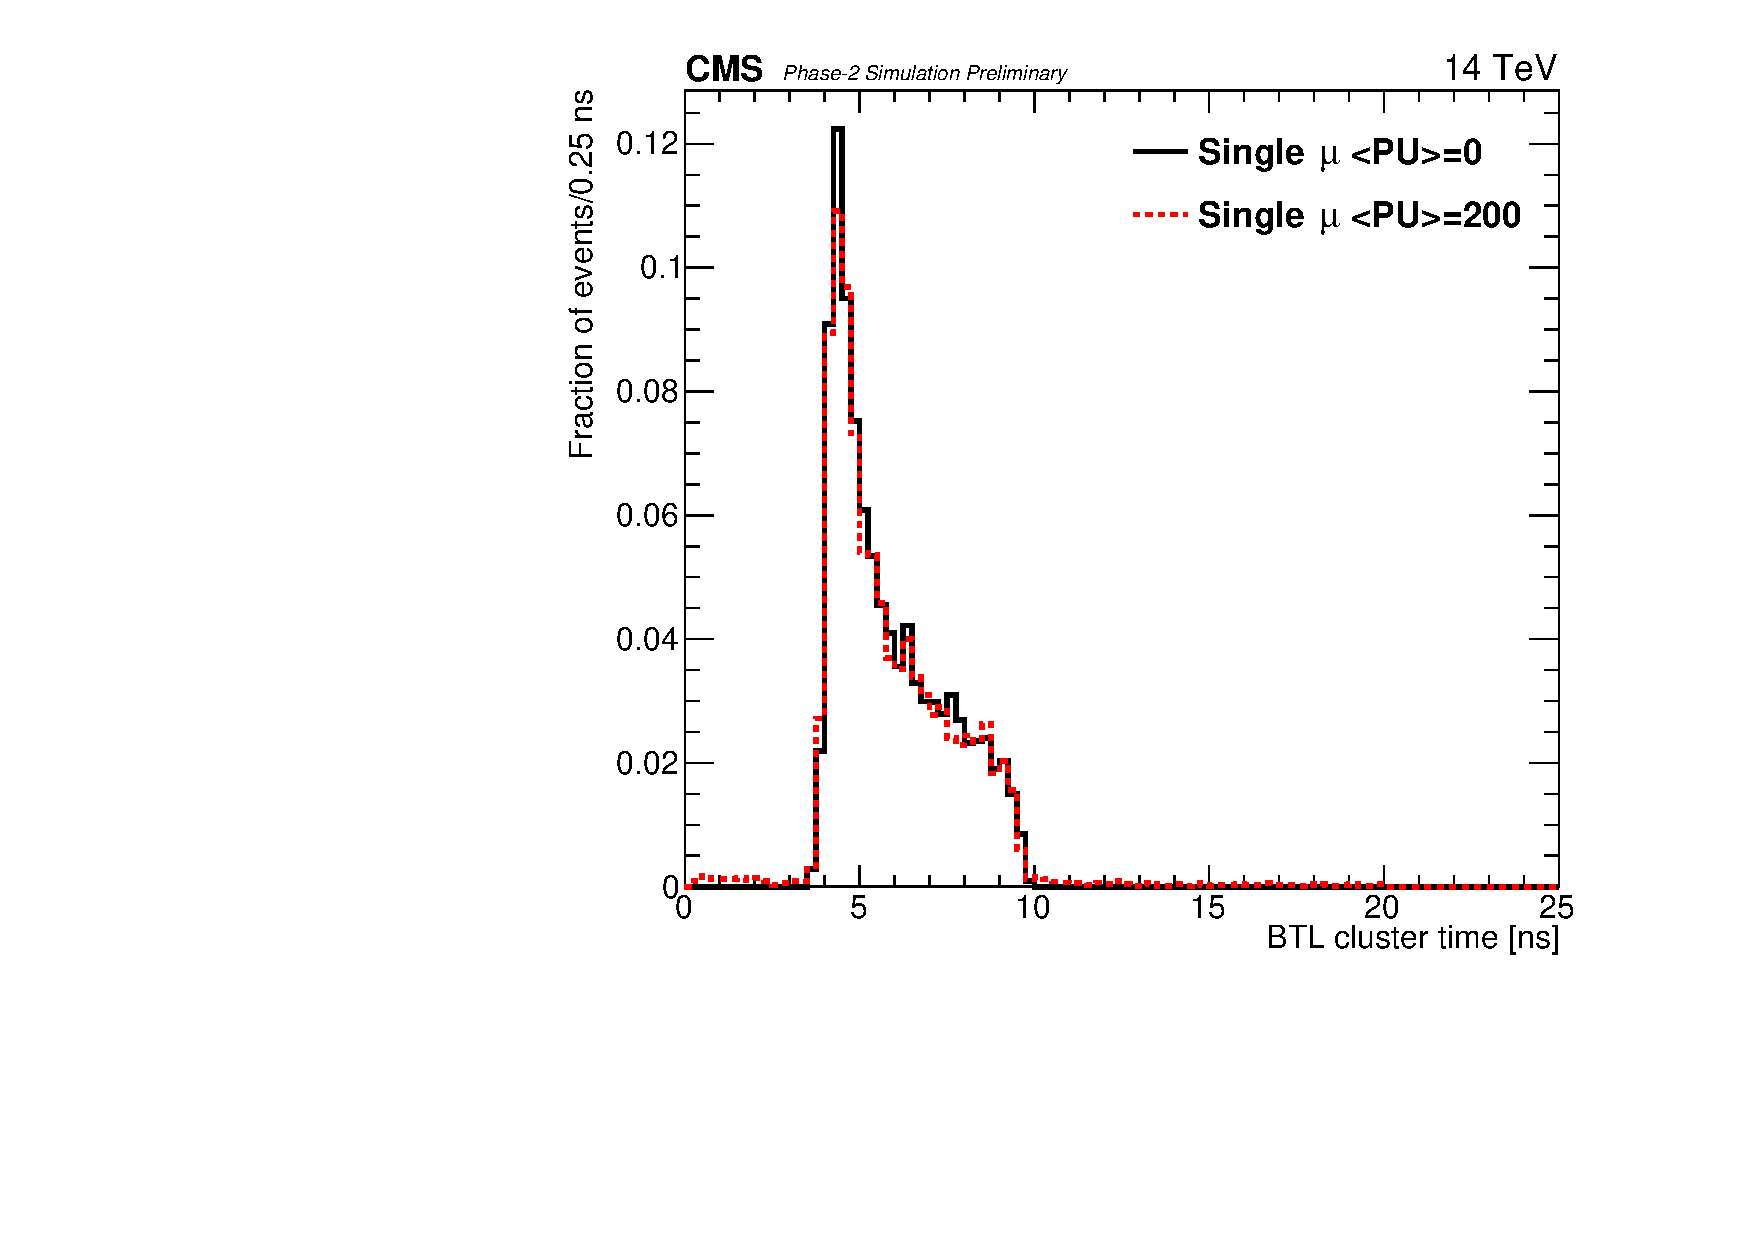
\includegraphics[width=0.48\textwidth]{fig/performance/ClusterAndTracks/BTLbestCluster_time_muPUcomp.pdf}
%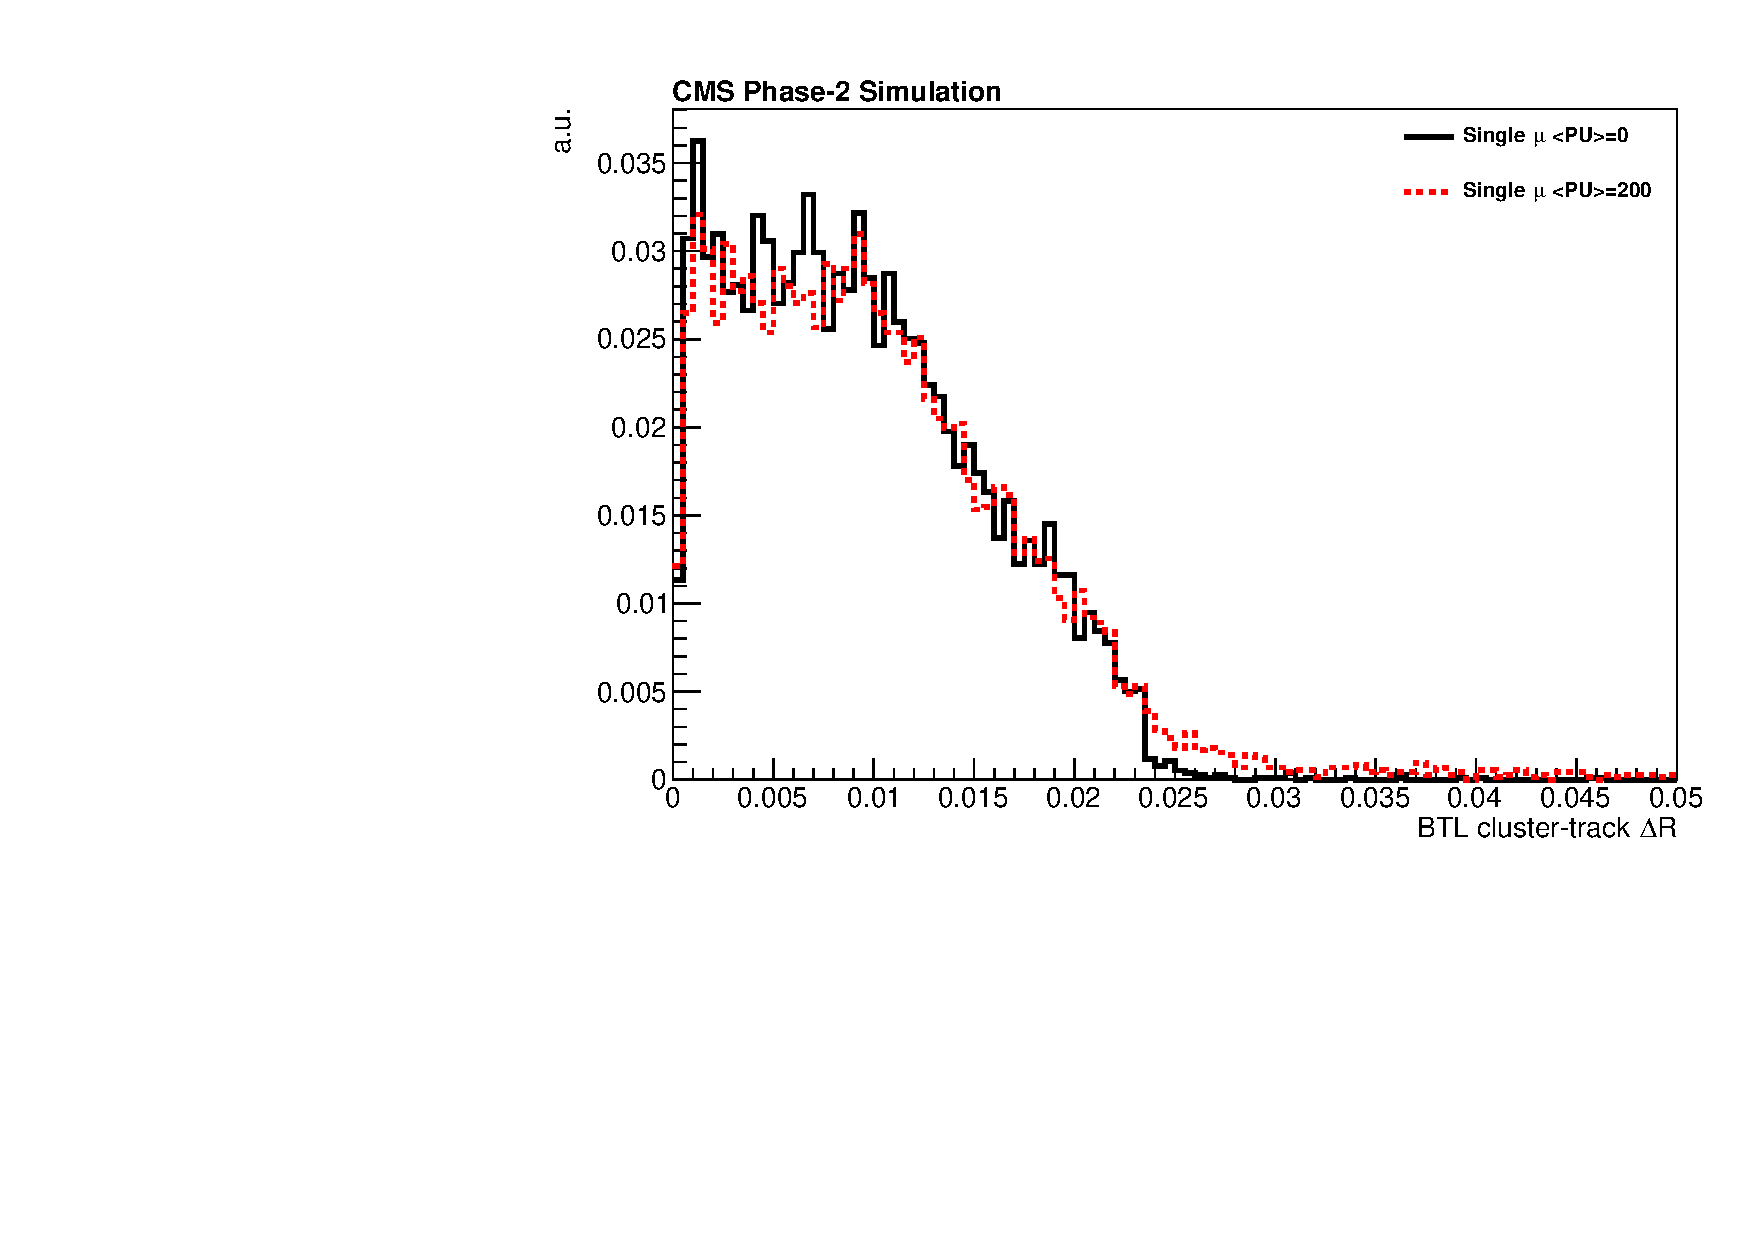
\includegraphics[width=0.32\textwidth]{fig/performance/ClusterAndTracks/BTLbestCluster_DR_muPUcomp.pdf}
\caption{Comparison of the BTL clusters size (left) and reconstructed time (right)
%and $\Delta R$ between the track propagated at the MTD and the cluster position
for single muon events (flat $p_{T}$ spectrum in 0.7-10~\mathrm{GeV} range) with an average of 200 pile-up events(red dotted line) and without pile-up (black line).}
\label{fig:clusterMuPuComp}
\end{figure}


\section{Time reconstruction for charged particles}

Tracks which have been reconstructed using the pixel detector and strip tracker are propagated to the MTD and spatially matched with compatible clusters.  If a compatible MTD cluster is found, the track parameters are then refit, including this as an additional spatial measurement.  The refitted track is then propagated from the point of closest approach to the beamline, to the MTD front surface, one tracking layer at a time in order to compute the total path length.  This path length is used together with the particle velocity based on the refitted momentum and using the pion mass hypothesis to correct the MTD cluster time back to the point of closest approach to the beamline.  

The efficiency for matching a reconstructed track to an MTD cluster as a function of $p_T$ and $\eta$ is shown in Figure \ref{fig:trackclusterefficiency} for single muon (with 200 average pile-up events and without pile-up) and single pion events in the acceptance region of the the MTD ($|\eta|<3$). Efficiency is flat as a function of $p_{T}$ (above 90\% for muons, around 80\% for pions), and reflects the different geometrical acceptance of the BTL and ETL. Efficiency for pions is also affected by nuclear interactions in the tracker volume as already discussed in section~\ref{sec:btlsim}.

\begin{figure}[!hbtp]
\centering
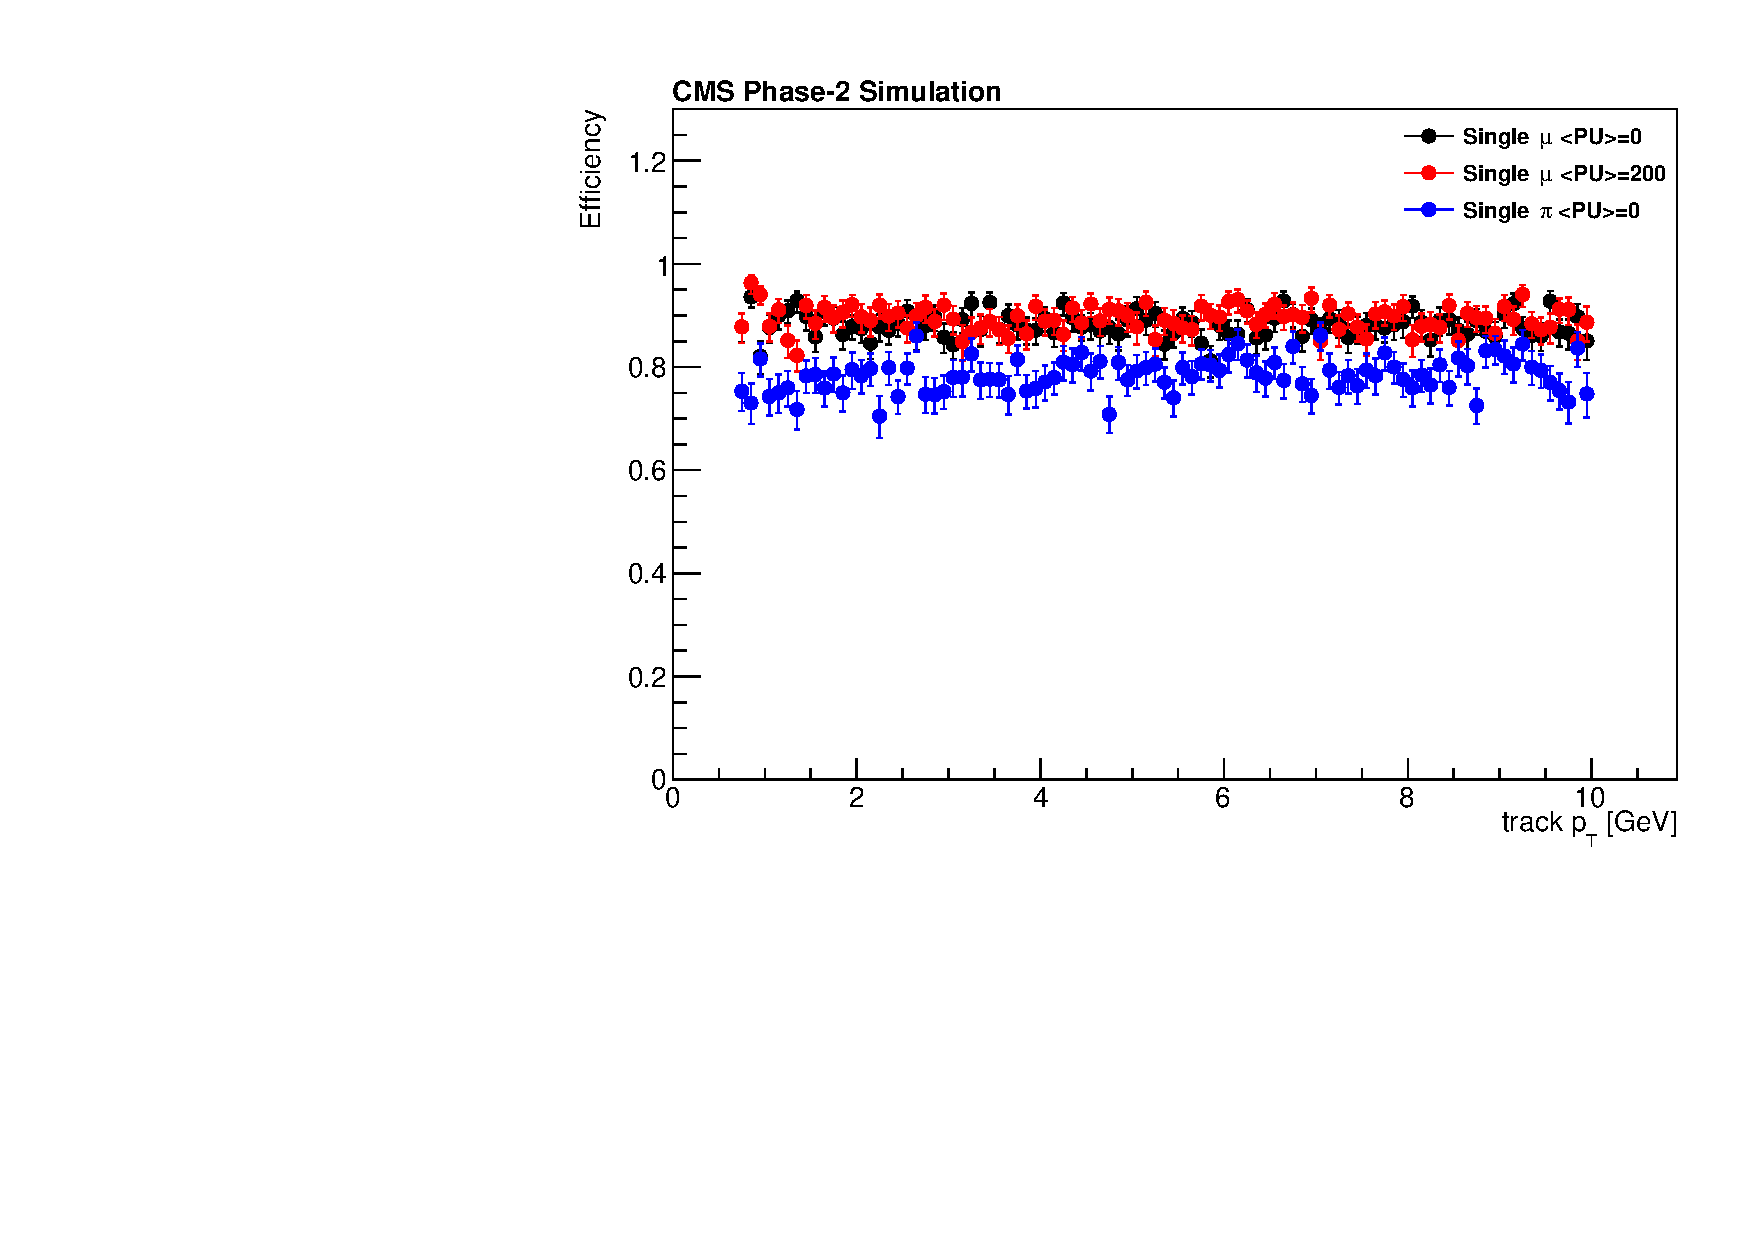
\includegraphics[width=0.48\textwidth]{fig/performance/ClusterAndTracks/divide_mtdTrack_pt_by_track_pt_mupiPUcomp.pdf}
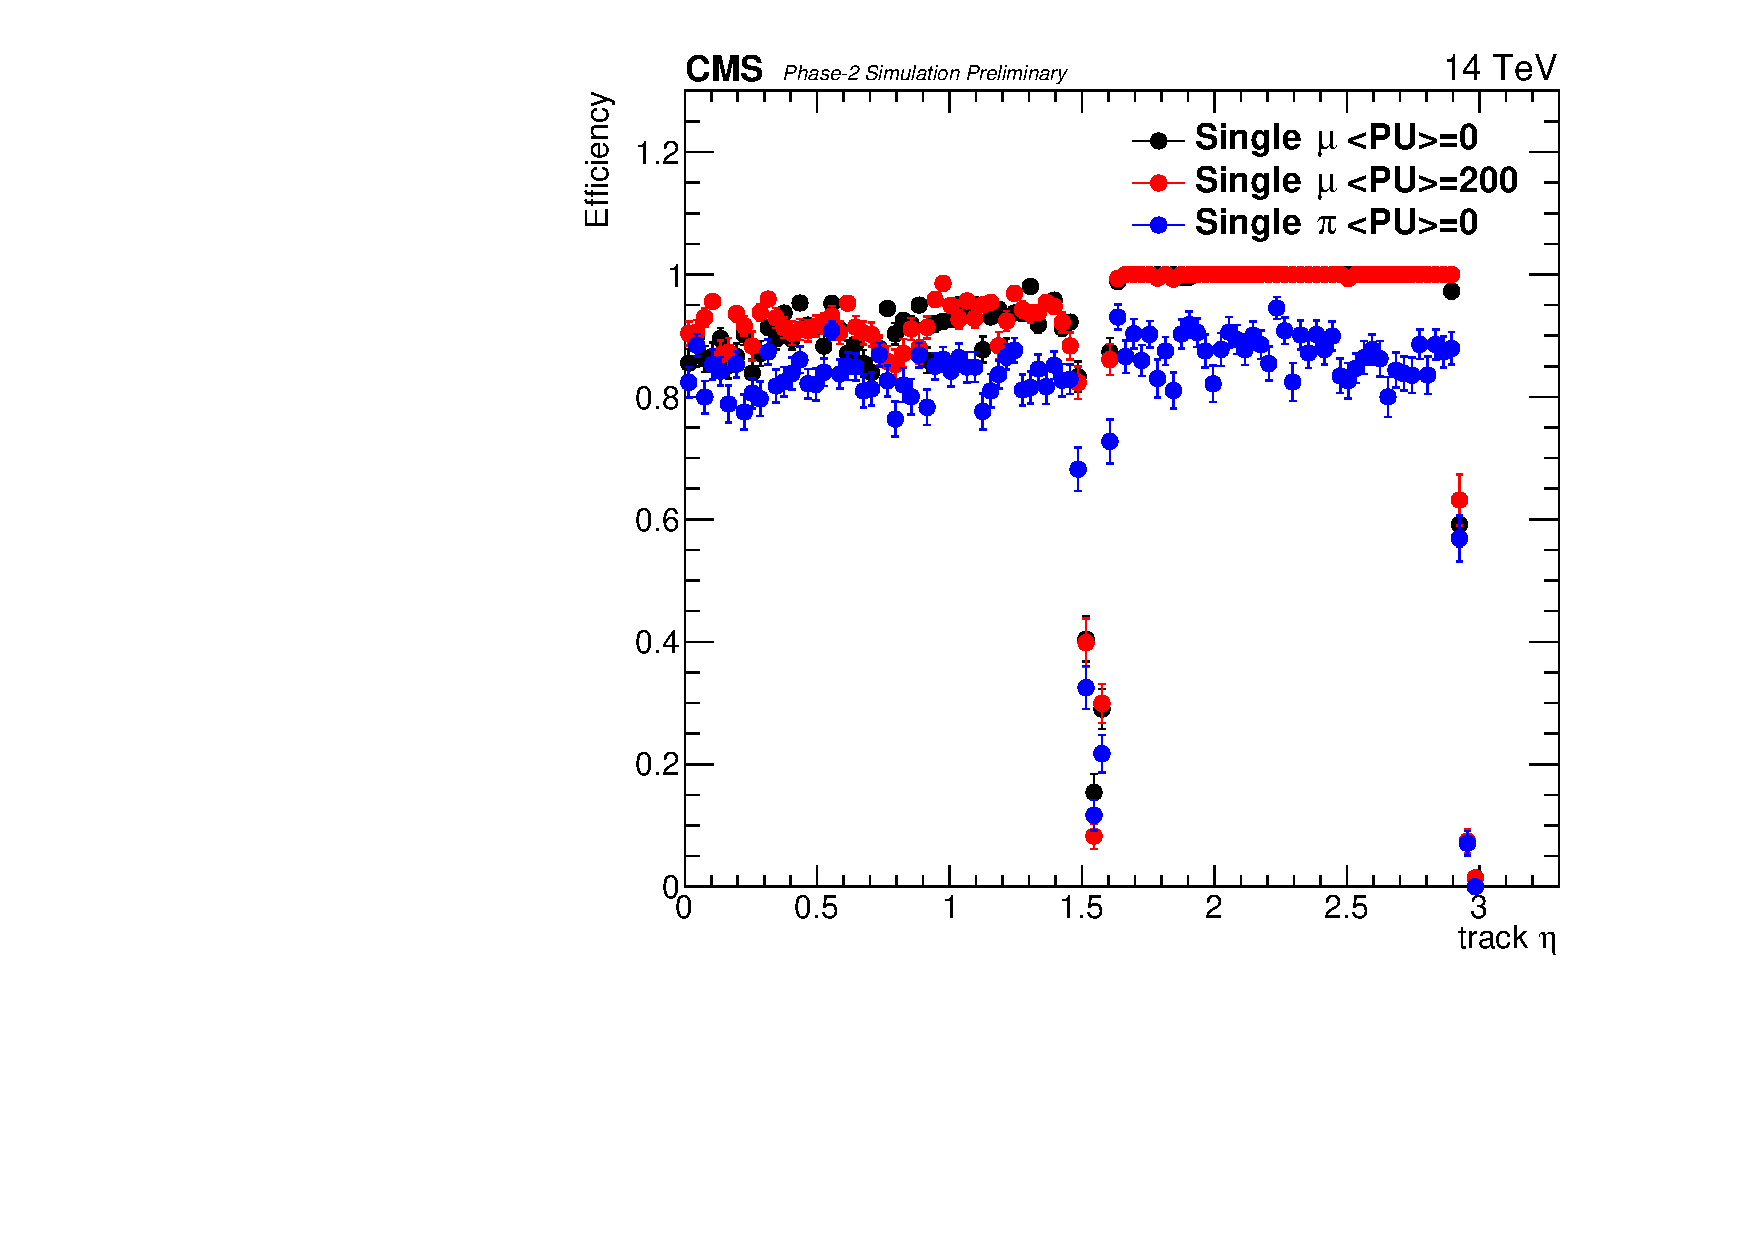
\includegraphics[width=0.48\textwidth]{fig/performance/ClusterAndTracks/divide_mtdTrack_eta_by_track_eta_mupiPUcomp.pdf}
\caption{Per-track efficiency to find an associated MTD cluster to a reconstructed track as a function of transverse momentum (left) and pseudo-rapidity (right). Tracks are matched to a generated particle in the event. Simulated particle gun events with a flat $p_T$ spectrum in the 0.7-10\mathrm{GeV} range are used. Muons (black and red dots are for events without pile-up and with average 200 pile-up events respectively) and pions (blue dots) are compared.}
\label{fig:trackclusterefficiency}
\end{figure}

The resulting time associated to the track and back-propagated to the beamline is compared to the simulation truth in Fig.~\ref{fig:trackt0vsgen}, using pions generated in simulated $t\bar{t}$ events at 14~\mathrm{TeV}. Tracks covering the BTL ($|\eta|<1.5$) and ETL ($1.5<|\eta|<3$) acceptance region are shown separately. From a fit to the distributions, the inferred time resolutions are 33~\mathrm{ps} and 35~\mathrm{ps} respectively for BTL and ETL, matching the expected simulated hit time resolutions. This also shows as expected that the track path-length estimation brings a negligible contribution to the time resolution.

\begin{figure}[!hbtp]
\centering
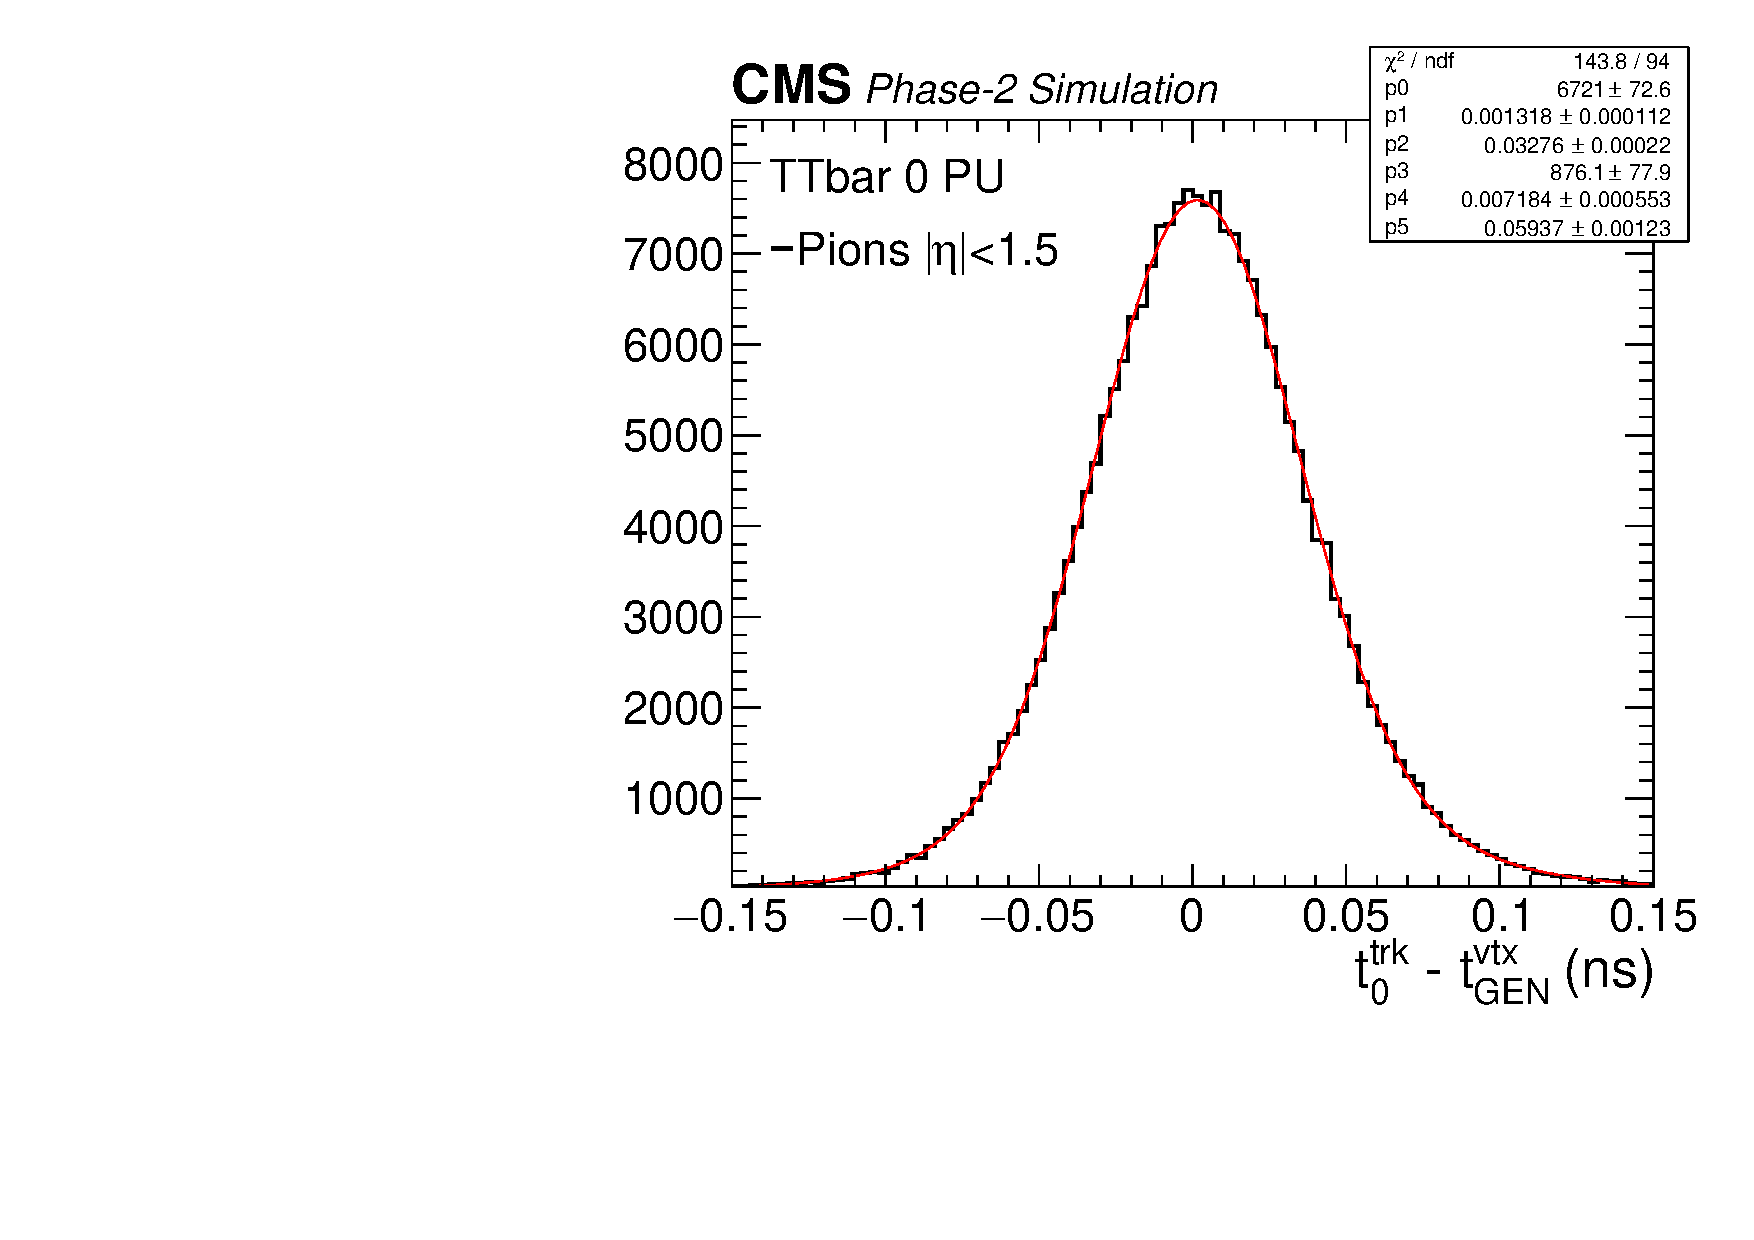
\includegraphics[width=0.48\textwidth]{fig/performance/ClusterAndTracks/res_t_pion_BTL.pdf}
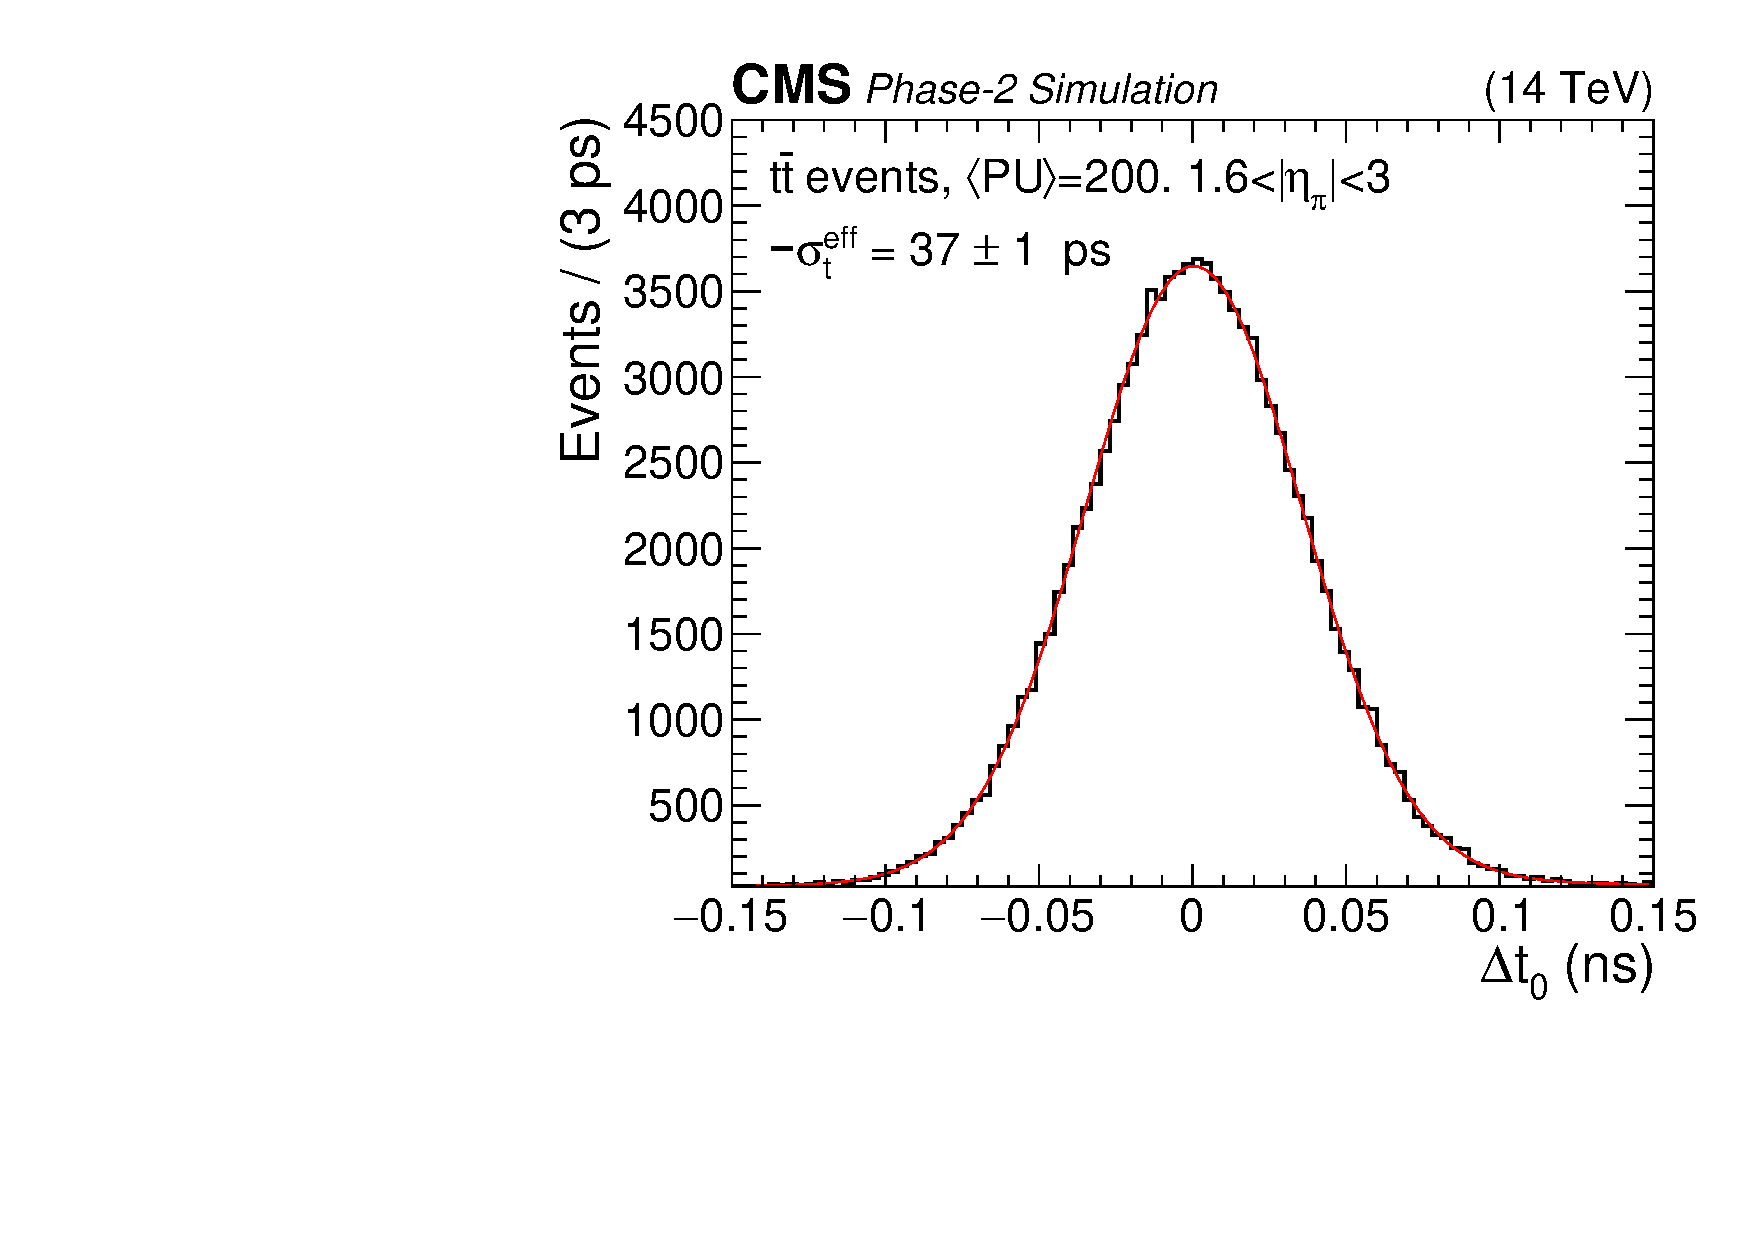
\includegraphics[width=0.48\textwidth]{fig/performance/ClusterAndTracks/res_t_pion_ETL.pdf}
\caption{Reconstructed track time at vertex respect to the simulation truth. Pions generated in simulated $t\bar{t}$ events at 14~\mathrm{TeV} are used. BTL (left) and ETL (right) acceptance regions are shown separately.}
\label{fig:trackt0vsgen}
\end{figure}

Time resolution for PU200 events in Fig.~\ref{fig:trackt0vsgen_PU200}, shows no degration of the achieved time resolution, with similar performance to the PU0 conditions.

\begin{figure}[!hbtp]
\centering
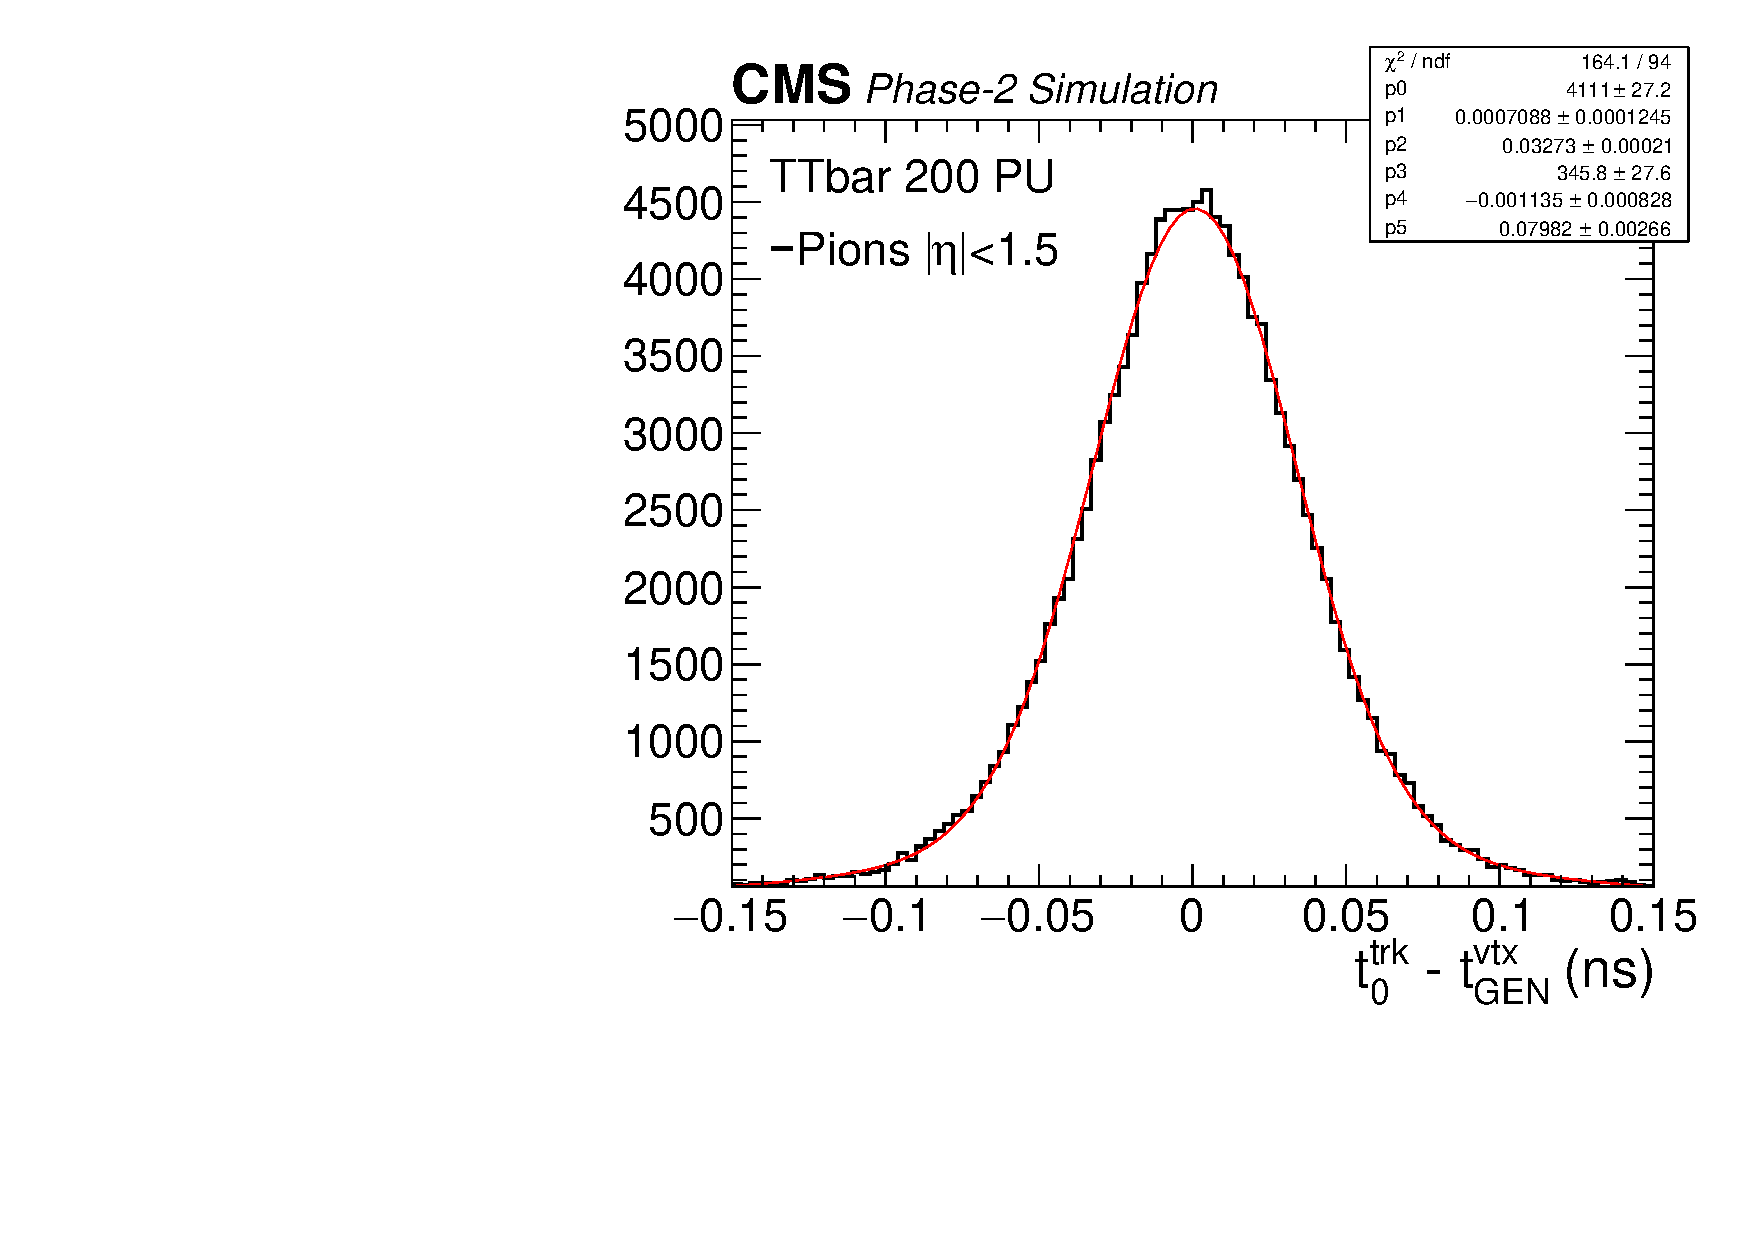
\includegraphics[width=0.48\textwidth]{fig/performance/ClusterAndTracks/res_t_pion_BTL_PU200.pdf}
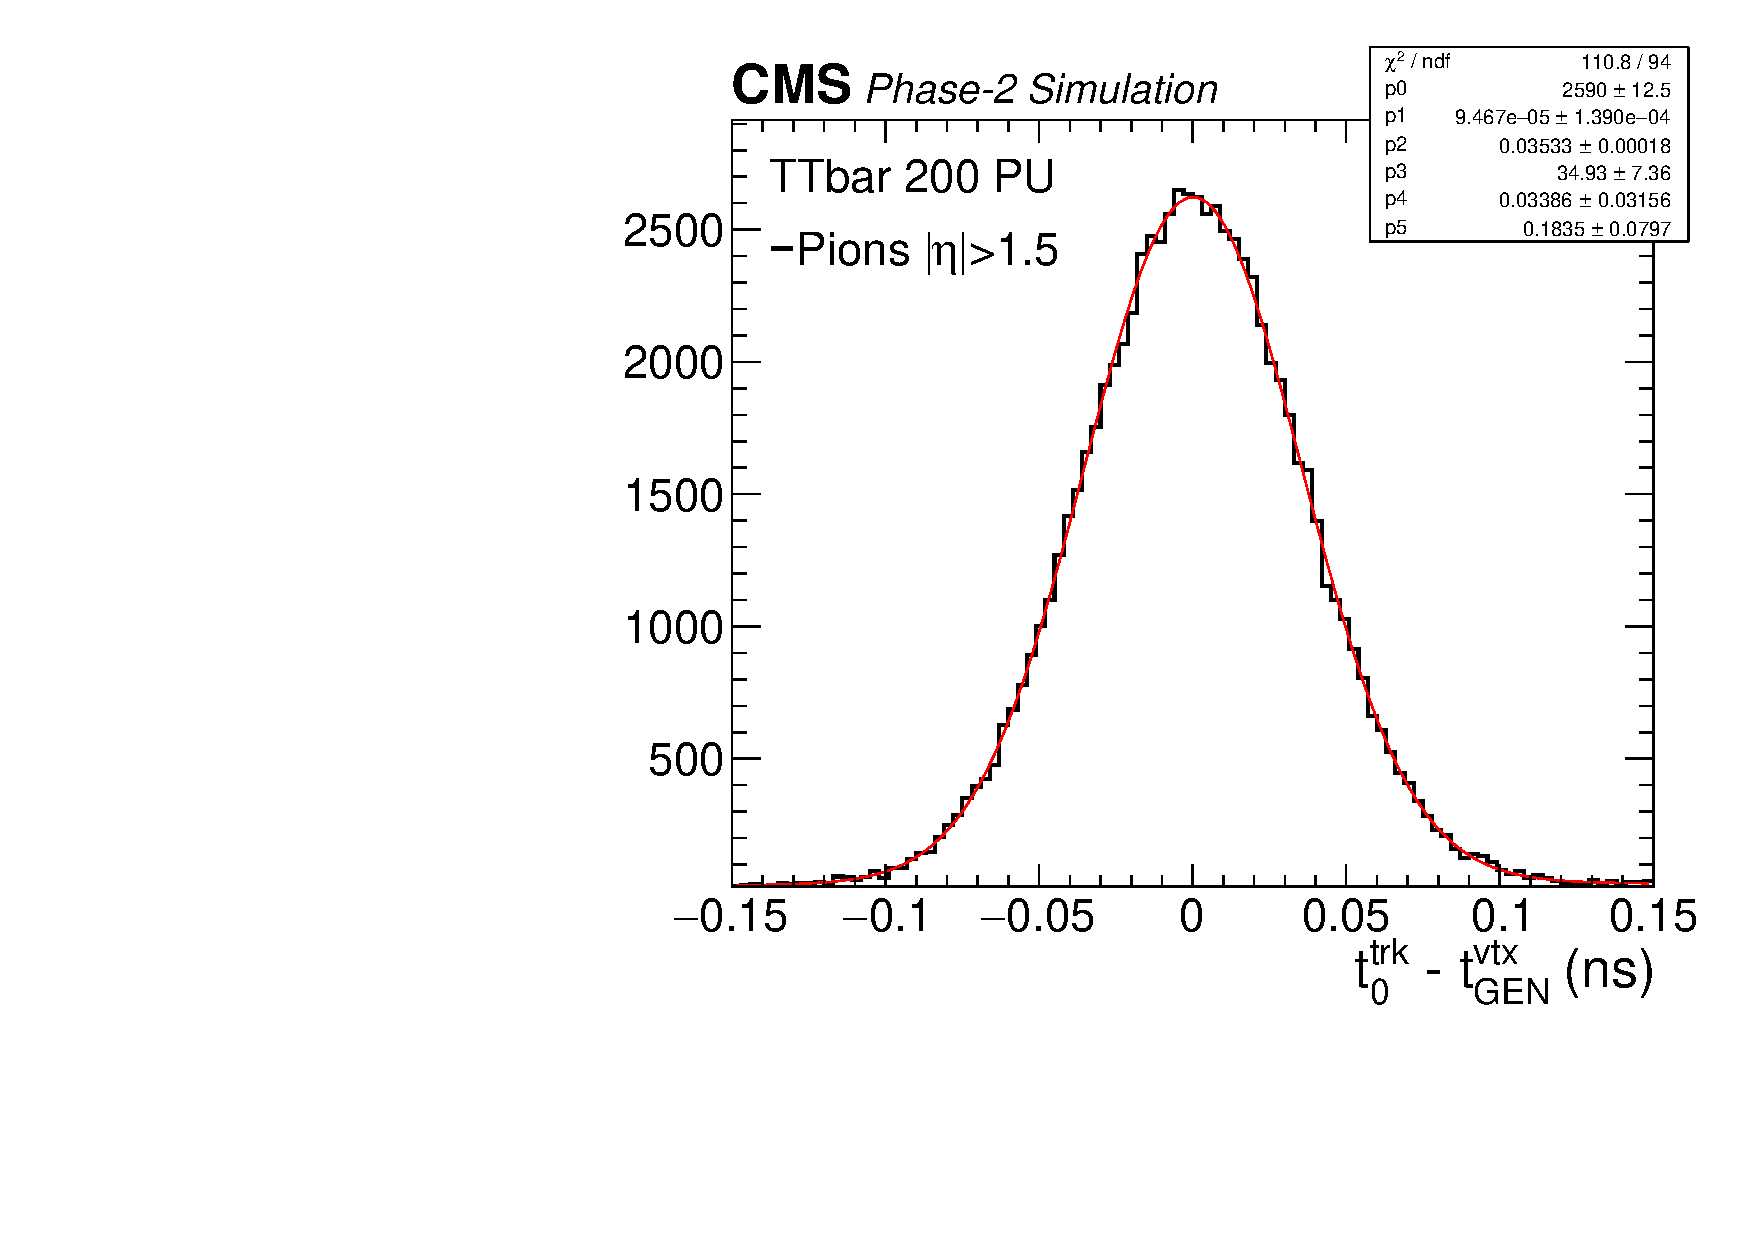
\includegraphics[width=0.48\textwidth]{fig/performance/ClusterAndTracks/res_t_pion_ETL_PU200.pdf}
\caption{Reconstructed track time at vertex respect to the simulation truth. Pions generated in simulated $t\bar{t}$ events at 14~\mathrm{TeV} are used. BTL (left) and ETL (right) acceptance regions are shown separately.}
\label{fig:trackt0vsgen_PU200}
\end{figure}

Fake hit association has been studied in DYJets events both without pile-up and at PU200. As we have seen fakes are not an issue for muon tracks which have a precise determination of the extrapolated position at the MTD surface (as signalled by having the same association efficiency for PU0 and PU200 events in Fig.~\ref{fig:trackclusterefficiency}). Fakes instead have a larger impact for low $p_{T}$ charged hadron tracks, as they typically have shorter tracks, with larger spatial extrapolation uncertainties.


In order to overcome this issue, different possibility for the hit association has been studied, foreseeing a possible iterative reconstruction for the MTD. Infact, knowing the time of vertex closest to the beam line propagation of the track, it is possible to infer using the track path-length the expected time at BTL. This allows to derive a time compatibility criteria which can be used for the hit association in addition to the space compatibility with the extrapolated track. In absence of the precise time determination for the vertex, the beam spot parameters can also be used as a constraint in the first reconstruction iteration, already with a substantial reduction of the combinatorics for PU200 events. Different mass hypothesis ($\pi,K,p$) can be considered to compute the track velocity when computing the time compatibility; the best mass hypothesis is used to define the matching criteria. 

In order to sort the hits a weighted $\chi^2=\chi^2_{space}+W\times\chi^2_{time}$ with $W=3$ is used. MTD matched tracks are defined to have with $\chi^2_{time}<5$ and  $\chi^2_{space}<50$. The weight $W$ and the matching criteria can be further optimised in the future, making them dependent on the track parameters ($p_{T},\eta,n_{hits},\dots$).  

Figure~\ref{fig:fakes} (left) shows the track-MTD association probability per track requiring that the back-propagated time to be within 3$\sigma$ from the vertex time as a function of $\eta$. Tracks are taken from  from DY events without pile-up and with PU200 and are required to have $p_{T}>0.7$~GeV and to be matched to a generator level particle. No requirement is applied to the track-quality. Different matching criteria are compared, showing that the fraction of tracks for which a good matching MTD hit has only a minor dependence on the matching criteria (somewhat indicating that for good reconstructed tracks the spatial matching is sufficient to identify the MTD hit position). The efficiency to associate the MTD hit remains unchanged going from PU0 to PU200, indicating that the occupancy of the MTD detector allows a good time reconstruction also in the high pile-up environment.   Figure~\ref{fig:fakes} (right) shows the probability per track to be associated to MTD but to have a back-propagated time above 3$\sigma$ from the vertex time, which is representative of the fake hit association. The different criteria shows a very different performance indicating that the vertex constraint play an important role in the reduction of the fake hits association in high pile-up environment. At the initial reconstruction step a beam spot constraint can be applied (the red-line) already with a large reduction of the fakes. A vertex constraint (blue line) can be applied in a second reconstruction step, perhaps applied only to the tracks sufficiently close to the primary vertex position in high pile-up environment and using the time of the closest reconstructed vertex position (in this study a 3mm cut is applied in the longitudinal direction). With a vertex constraint, both the association efficiency and fake rate can be maintained to levels which are close between PU0 and PU200.

\begin{figure}[!hbtp]
\centering
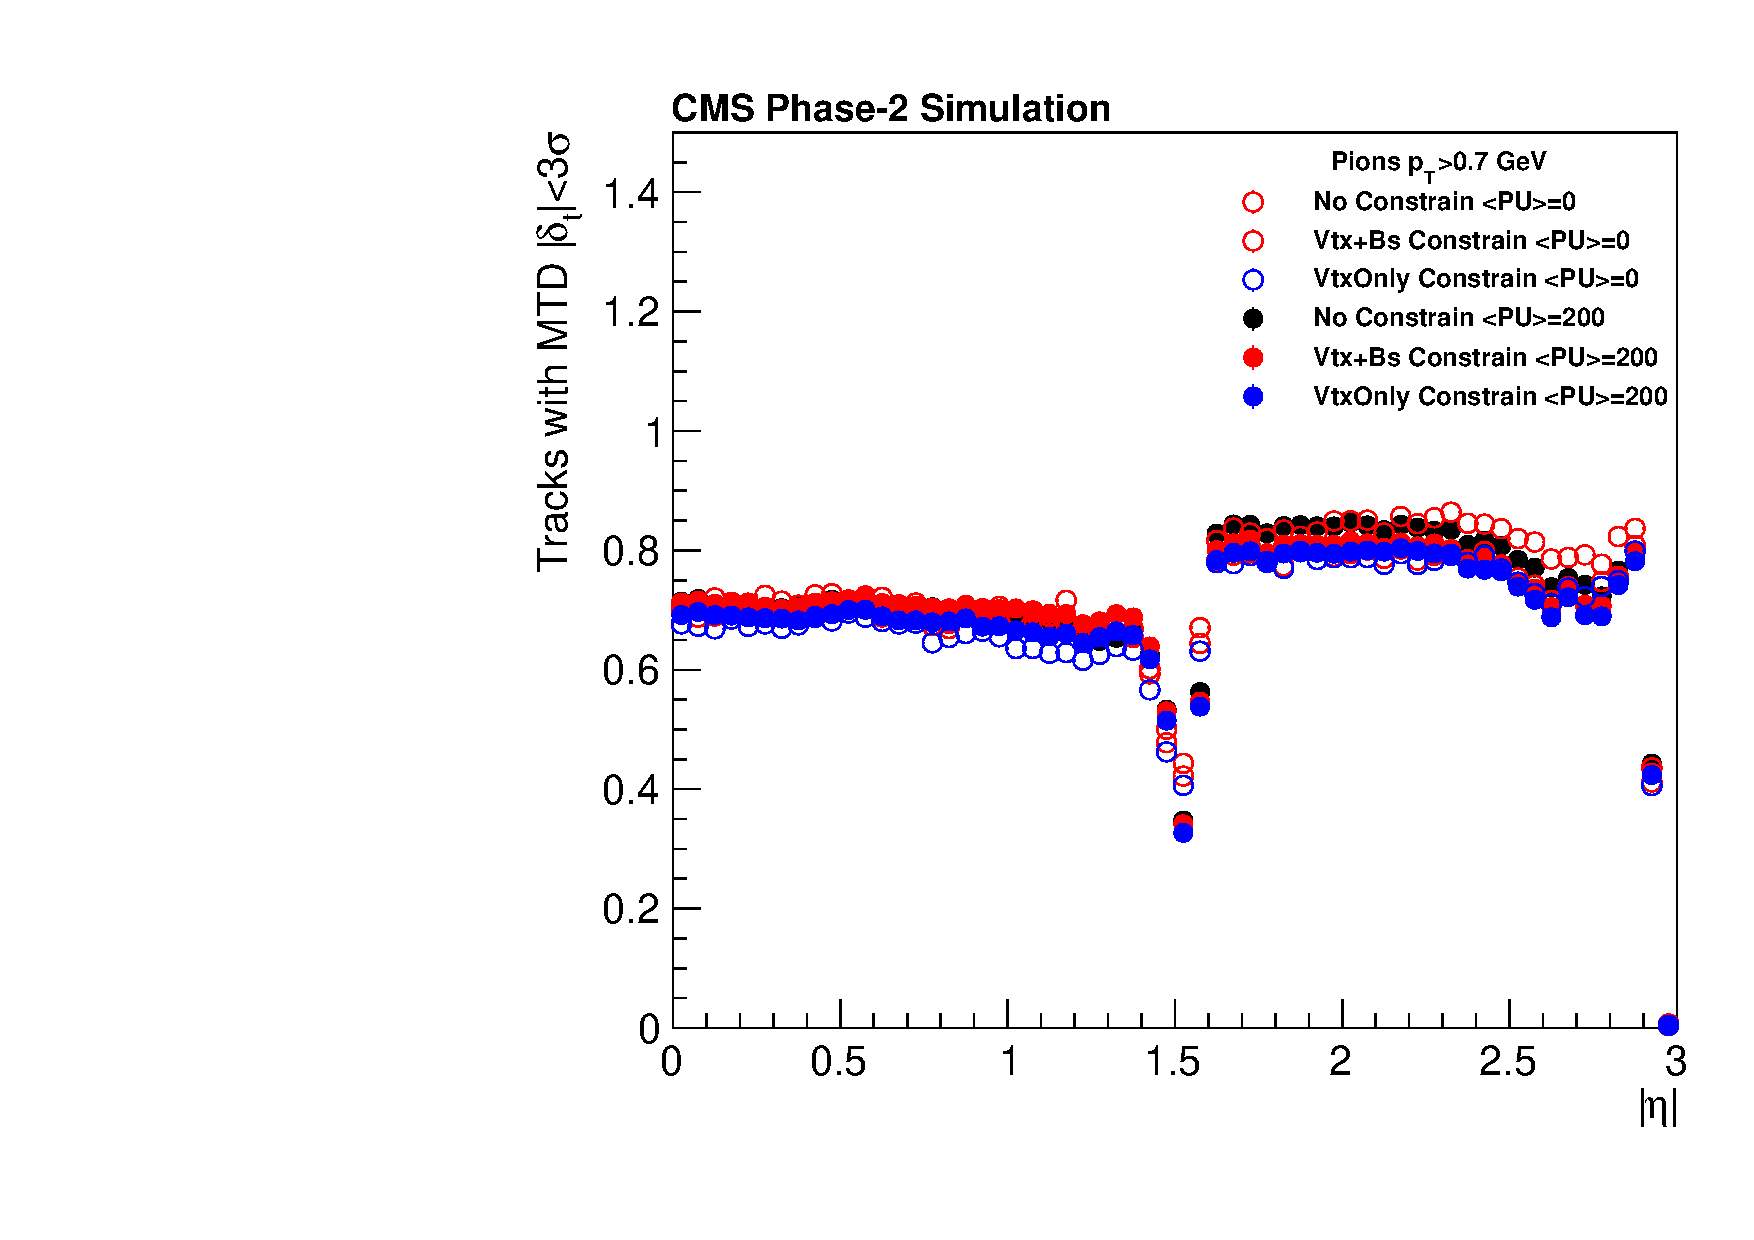
\includegraphics[width=0.48\textwidth]{fig/performance/goodTracks_vs_eta_fullComp.pdf}
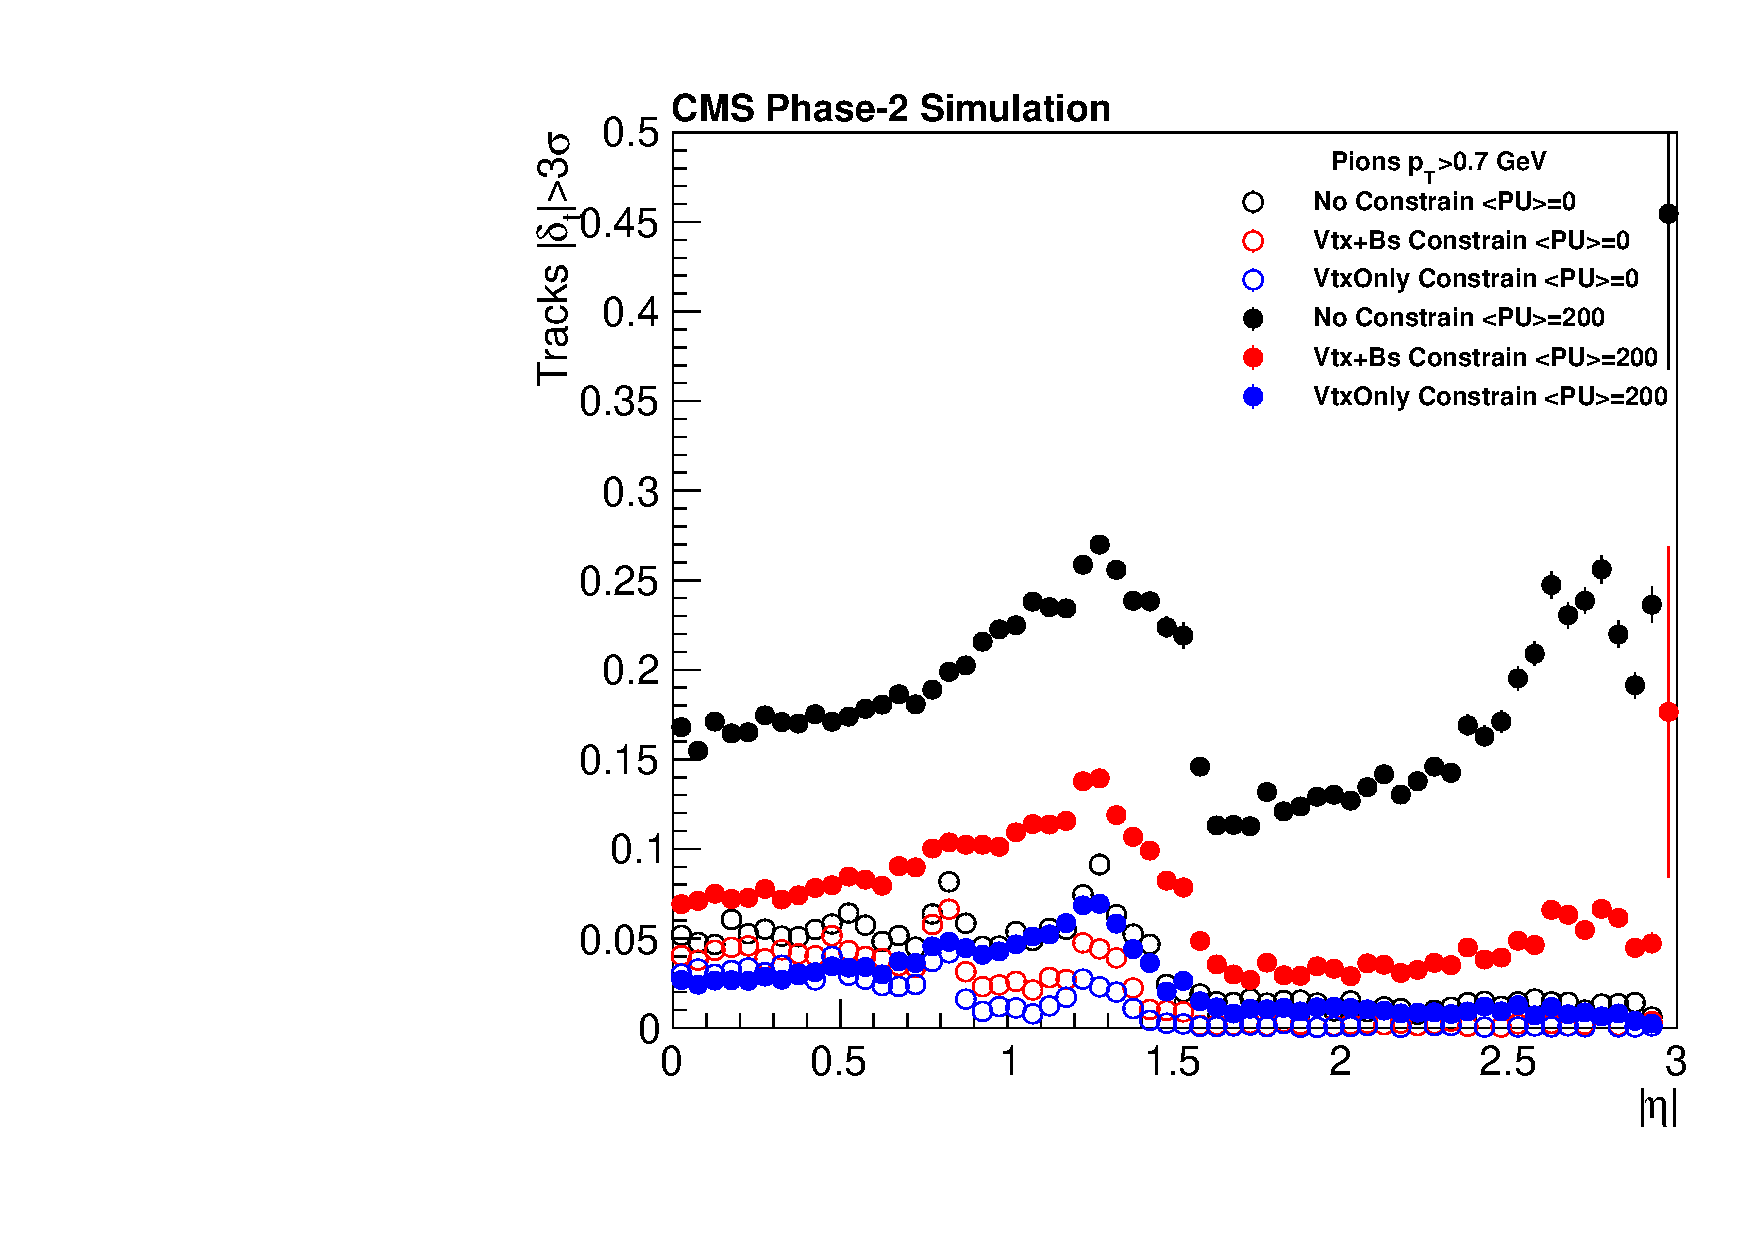
\includegraphics[width=0.48\textwidth]{fig/performance/fakes_vs_eta_fullComp.pdf}
\caption{Probability per track as a function of the pseudo-rapidity to find a good association with MTD ($\delta_{t}^{vtx}<3\sigma$, left) and a wrong association ($\delta_{t}^{vtx}>3\sigma$, right). Tracks are taken from  from DY events without pile-up and with PU200 and are required to have $p_{T}>0.7$~GeV and to be matched to a generator level particle. No requirement is applied to the track-quality. Different matching criteria are used: black only spatial matching, red time and space matching with a beam spot constrain, blue time and space matching with vertex constrain. See text for more details}
\label{fig:fakes}
\end{figure}

Fake rates are also shown as a function of track $p_{T}$ (left) and track number of hits (right) in Fig.\ref{fig:fakes_pt_nhits}. This shows that the fake rate is not an issue when track extrapolation has a good precision, indicating that the fakes can be further reduced from an optimisation of the track reconstruction at PU200 focussed on low $p_{T}$ hadrons. 

\begin{figure}[!hbtp]
\centering
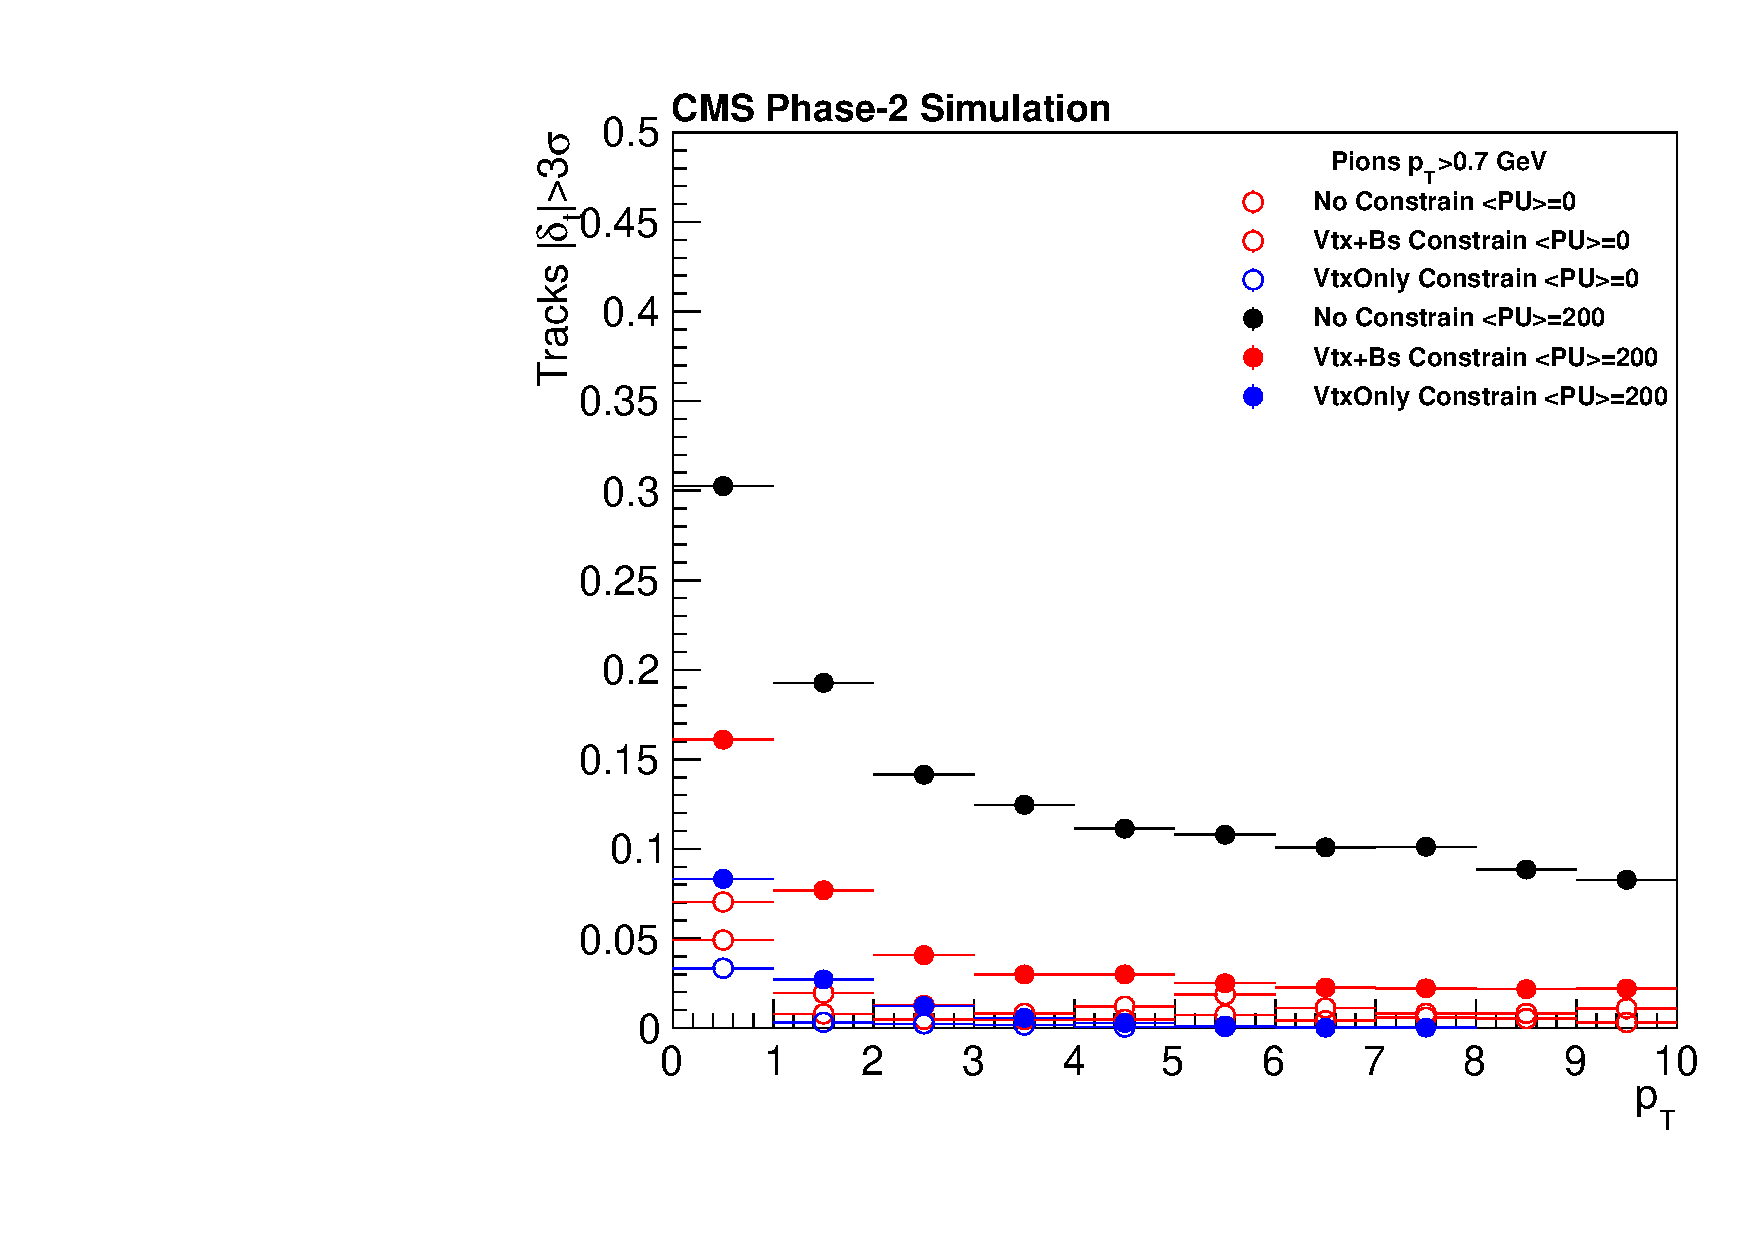
\includegraphics[width=0.48\textwidth]{fig/performance/fakes_vs_pt_fullComp.pdf}
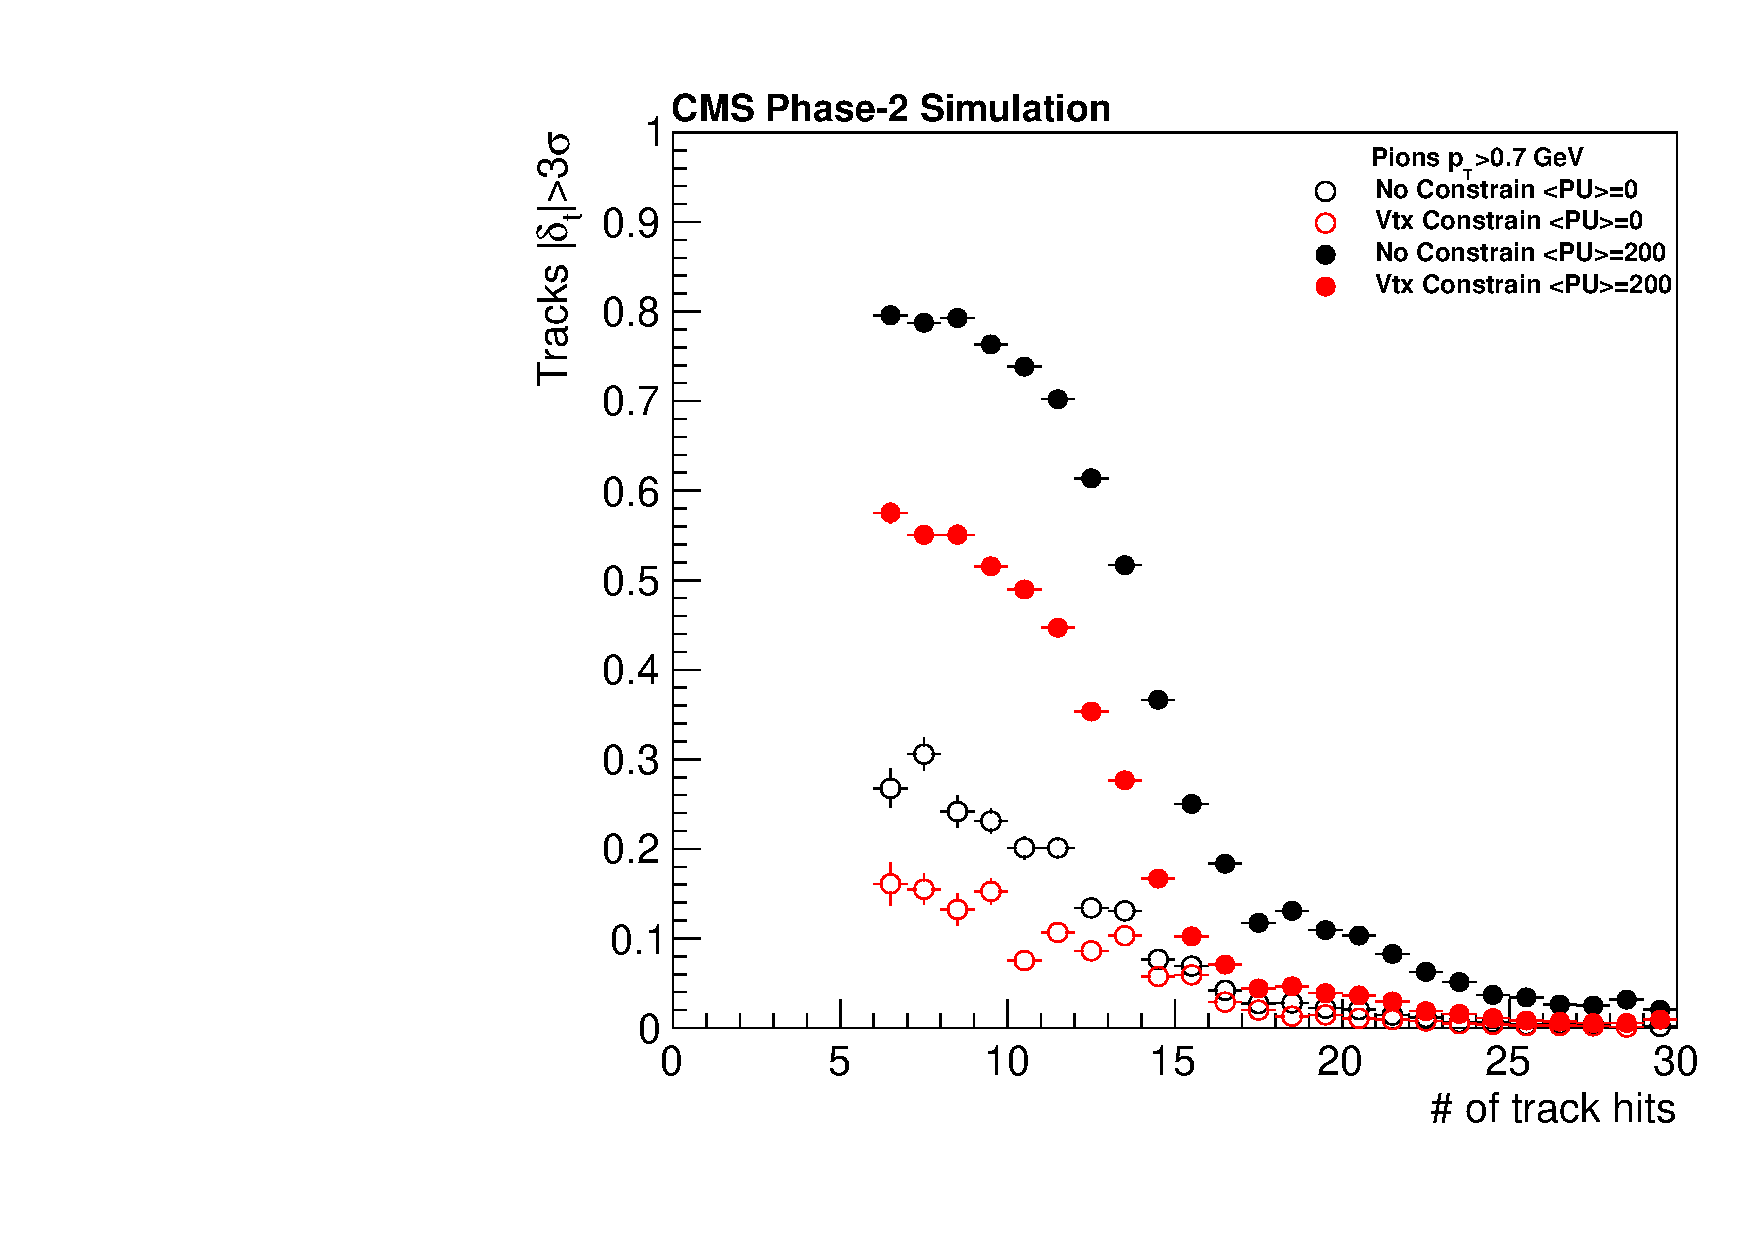
\includegraphics[width=0.48\textwidth]{fig/performance/fakes_vs_nHits.pdf}
\caption{Probability per track as a function of the $p_{T}$ (left) and number of track hits (right) to have a wrong association with MTD ($\delta_{t}^{vtx}>3\sigma$). Tracks are taken from  from DY events without pile-up and with PU200 and are required to have $p_{T}>0.7$~GeV and to be matched to a generator level particle. No requirement is applied to the track-quality. Different matching criteria are used: black only spatial matching, red time and space matching with a beam spot constrain, blue time and space matching with vertex constrain. See text for more details}
\label{fig:fakes_pt_nhits}
\end{figure}

For analysis purposes, tracks can be selected to further reduce the fake contributions (e.g requiring a minimum number of hits). As we will see in the PU rejection studies, these criteria can be further developed implementing a multivariate classifier, feeded with track quality variables and track-MTD matching criteria.


\section{Time reconstruction for converted photons}
\section{4D vertex reconstruction}
\section{Pile-up tracks rejection using timing informations}
An essential step in rejecting pileup is to exclude from relevant
quantities charged particles which are not associated with the hard
interaction.  
This step is critical to maintain the performance of charged isolation
sums for leptons, b-tagging, and the charged component of jets and
missing transverse momentum.  
One method commonly used in CMS  to associate tracks with the hard
primary vertex, PV, is a simple selection on the distance between the
track and the vertex, $|\Delta
z(\textnormal{track},\textnormal{PV})|<1$~mm, which maintains 
high efficiency for charged particles actually originating from the
hard interaction. 
To optimize this seleciton, the isolation sum of charged
particles was studied in 200 pileup collisions for $|\Delta z|$
ranging between 0.2 and 2~mm. 
For particles at any pseudorapidity within the barrel acceptance, a
selection window of 1~mm maximizes the identification performance
(measured by the ROC curve).  
In the endcaps, a slightly looser selection may provide a better
performance, with 1~mm being close to optimal. 
Hence, for an interaction density in excess of 1.0~event/mm,
corresponding to operations at approximately 100 pileup and above,
some or many of the resulting tracks will be associated with the 
hard primary vertex, contaminating the set of tracks used to calculate
the relevant physics quantities and degrading the performance.

This effect is most directly quantified as a function of the line
density of events along the beam line, which drives the probability
that additional vertices will be close enough in space to the hard
interaction to contaminate the set of associated tracks with those
from pileup. 
This association method can be extended with precision timing, by
adding a requirement on the time distance $|\Delta
t(\textnormal{track},\textnormal{PV})|<N\times\sigma_t^{\textnormal{track}}$ for those tracks with valid timing information.  Tracks without valid timing information are retained.
In this study,  $N = 3$ is used together with an average time resolution $\sigma_t=35$~ps for tracks with valid timing information, corresponding to the requirement 
$|\Delta t(\textnormal{track},\textnormal{PV})|<105$~ps.

Using this association criterion, the efficiency for reconstructing and
associating tracks from pileup interactions in \ttbar events is
shown in Fig.~\ref{fig:trkvtx}, both with and without precision
timing, as a function of the event line density. The effect of timing
on signal tracks for these processes  has been studied as well, and in
zero-pileup conditions shows no significant impact on the association
efficiency. 

The left panel of the figure shows the results obtained with the full
simulation and reconstruction described in this TDR, while the right
panel shows results from the fast-simulation, where the time smearing
is applied at the vertex. A fair agreement is observed in the
reduction of wrong associations for comparable assumption on the
timing resolution. This provides confidence in the use of the fast
simulation adopted for some of the performance analyses presented in
the next sections.  

\begin{figure}[hbtp]
\centering
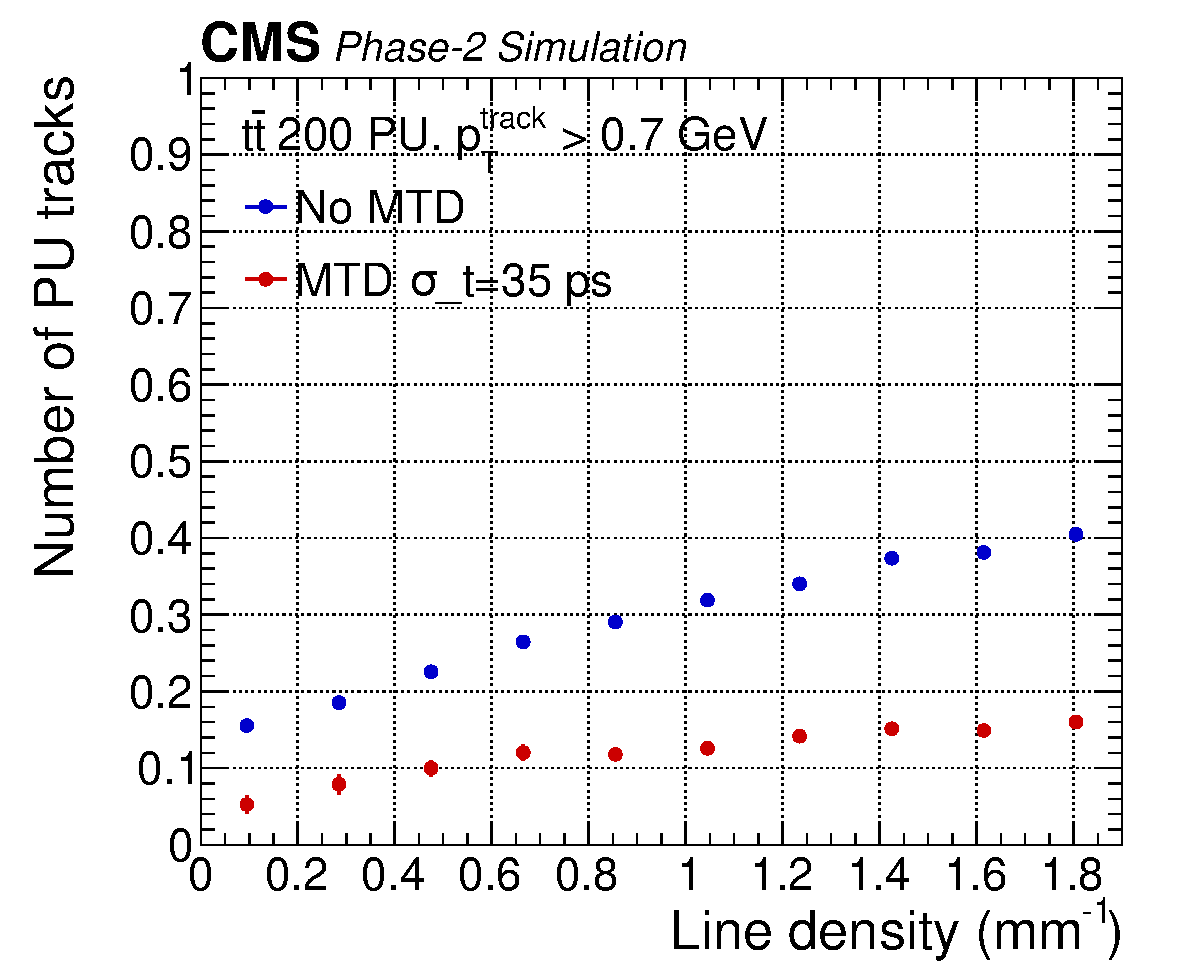
\includegraphics[width=0.52\textwidth]{fig/performance/trkvtx/track_pu_vs_linden_s.pdf}
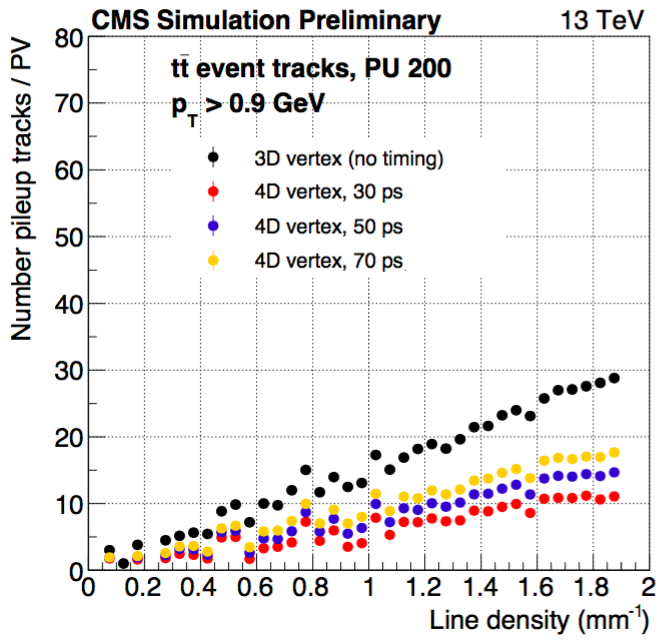
\includegraphics[width=0.44\textwidth]{fig/performance/trkvtx/nPUTracks_fromNtuple_tres.png}
 \caption{Left: Fraction of tracks from pileup incorrectly 
   associated with the hard primary vertex in \ttbar events from full
   simulation as a function of the pileup density, shown with (4D vtx)
   and without (3D vtx) precision timing. Right: Ditto for
   fast-simulation and different assumption on the timing resolution.}
   \label{fig:trkvtx}
\end{figure}

\end{document}
